%----------------------------------------------------------------------------------------
%	PACKAGES AND OTHER DOCUMENT CONFIGURATIONS
%----------------------------------------------------------------------------------------

\documentclass[
    11pt,
%oneside, % Two side (alternating margins) for binding by default, uncomment to switch to one side
    english, % ngerman for German
    singlespacing, % Single line spacing, alternatives: onehalfspacing or doublespacing
%draft, % Uncomment to enable draft mode (no pictures, no links, overfull hboxes indicated)
%nolistspacing, % If the document is onehalfspacing or doublespacing, uncomment this to set spacing in lists to single
%liststotoc, % Uncomment to add the list of figures/tables/etc to the table of contents
%toctotoc, % Uncomment to add the main table of contents to the table of contents
%parskip, % Uncomment to add space between paragraphs
%nohyperref, % Uncomment to not load the hyperref package
    headsepline, % Uncomment to get a line under the header
%chapterinoneline, % Uncomment to place the chapter title next to the number on one line
%consistentlayout, % Uncomment to change the layout of the declaration, abstract and acknowledgements pages to match the default layout
    oneside, % uncomment for clear page spacing between sections
]{MastersDoctoralThesis} % The class file specifying the document structure

\usepackage[utf8]{inputenc} % Required for inputting international characters
\usepackage[T1]{fontenc} % Output font encoding for international characters
\usepackage{float}% If comment this, figure moves to Page 2
\usepackage{spverbatim}

\usepackage{mathpazo} % Use the Palatino font by default

\usepackage[backend=bibtex,style=authoryear,natbib=true]{biblatex} % Use the bibtex backend with the authoryear citation style (which resembles APA)

\addbibresource{main.bib} % The filename of the bibliography

\usepackage[autostyle=true]{csquotes} % Required to generate language-dependent quotes in the bibliography


%----------------------------------------------------------------------------------------
%	MARGIN SETTINGS
%----------------------------------------------------------------------------------------

\geometry{
    paper=a4paper, % Change to letterpaper for US letter
    inner=2.5cm, % Inner margin
    outer=3.8cm, % Outer margin
    bindingoffset=.5cm, % Binding offset
    top=1.5cm, % Top margin
    bottom=1.5cm, % Bottom margin
%showframe, % Uncomment to show how the type block is set on the page
}

%----------------------------------------------------------------------------------------
%	THESIS INFORMATION
%----------------------------------------------------------------------------------------

\thesistitle{The Mango Messenger} % Your thesis title, this is used in the title and abstract, print it elsewhere with \ttitle
\supervisor{Dr. Szymon Murawski} % Your supervisor's name, this is used in the title page, print it elsewhere with \supname
\examiner{} % Your examiner's name, this is not currently used anywhere in the template, print it elsewhere with \examname
\degree{Bachelor of Computer Science} % Your degree name, this is used in the title page and abstract, print it elsewhere with \degreename
\author{Petro Kolosov, Serhii Holishevskyi, Illia Zubachov, Arslanbek Temirbekov} % Your name, this is used in the title page and abstract, print it elsewhere with \authorname
\addresses{} % Your address, this is not currently used anywhere in the template, print it elsewhere with \addressname

\subject{Biological Sciences} % Your subject area, this is not currently used anywhere in the template, print it elsewhere with \subjectname
\keywords{} % Keywords for your thesis, this is not currently used anywhere in the template, print it elsewhere with \keywordnames
\university{Wyzsza Szkola Bankowa w Poznaniu} % Your university's name and URL, this is used in the title page and abstract, print it elsewhere with \univname
\department{Department of Computer Science} % Your department's name and URL, this is used in the title page and abstract, print it elsewhere with \deptname
\group{Wyzsza Szkola Bankowa w Poznaniu} % Your research group's name and URL, this is used in the title page, print it elsewhere with \groupname
\faculty{Computer Science} % Your faculty's name and URL, this is used in the title page and abstract, print it elsewhere with \facname

\AtBeginDocument{
    \hypersetup{pdftitle=\ttitle} % Set the PDF's title to your title
    \hypersetup{pdfauthor=\authorname} % Set the PDF's author to your name
    \hypersetup{pdfkeywords=\keywordnames} % Set the PDF's keywords to your keywords
}

\begin{document}

    \frontmatter % Use roman page numbering style (i, ii, iii, iv...) for the pre-content pages

    \pagestyle{plain} % Default to the plain heading style until the thesis style is called for the body content

%----------------------------------------------------------------------------------------
%	TITLE PAGE
%----------------------------------------------------------------------------------------

    \begin{titlepage}
        \begin{center}
            
\includegraphics[width=0.5\textwidth]{wsb_logo} \\ % University/department logo - uncomment to place it
            \vspace*{.06\textheight}
            {\scshape\LARGE \univname\par}\vspace{1.5cm} % University name
            \textsc{\Large Bachelor Thesis}\\[0.5cm] % Thesis type

            \HRule \\[0.4cm] % Horizontal line
            {\huge \bfseries \ttitle\par}\vspace{0.4cm}
            \HRule \\[1.5cm] % Horizontal line

            \begin{minipage}[t]{0.4\textwidth}
                \begin{flushleft}
                    \large
                    \emph{Authors:}\\
                    \authorname % Author name - remove the \href bracket to remove the link
                \end{flushleft}
            \end{minipage}
            \begin{minipage}[t]{0.4\textwidth}
                \begin{flushright}
                    \large
                    \emph{Supervisor:} \\
                    \supname % Supervisor name - remove the \href bracket to remove the link
                \end{flushright}
            \end{minipage}\\[3cm]

            \vfill

            \large \textit{A thesis submitted in fulfillment of the requirements\\ for the degree of \degreename}\\[0.3cm] % University requirement text
            \textit{in the}\\[0.4cm]
            \groupname\\\deptname\\[2cm] % Research group name and department name

            \vfill

            {\large \today}\\[4cm] % Date

            \vfill
        \end{center}
    \end{titlepage}

%----------------------------------------------------------------------------------------
%	DECLARATION PAGE
%----------------------------------------------------------------------------------------

    \begin{declaration}
        \addchaptertocentry{\authorshipname} % Add the declaration to the table of contents
        \noindent We, \authorname, declare that this thesis titled, \enquote{\ttitle} and the work presented in it are my own.
        We confirm that:

        \begin{itemize}
            \item This work was done wholly or mainly while in candidature for a research degree at this University.
            \item Where any part of this thesis has previously been submitted for a degree or any other qualification at this University or any other institution, this has been clearly stated.
            \item Where I have consulted the published work of others, this is always clearly attributed.
            \item Where I have quoted from the work of others, the source is always given.
            With the exception of such quotations, this thesis is entirely my own work.
            \item I have acknowledged all main sources of help.
            \item Where the thesis is based on work done by myself jointly with others, I have made clear exactly what was done by others and what I have contributed myself.\\
        \end{itemize}

        \noindent Signed:\\
        \rule[0.5em]{25em}{0.5pt} % This prints a line for the signature

        \noindent Date:\\
        \rule[0.5em]{25em}{0.5pt} % This prints a line to write the date
    \end{declaration}

%----------------------------------------------------------------------------------------
%	PARTNER DETAILS PAGE
%----------------------------------------------------------------------------------------
    \begin{partnerdetailspage}
        \textbf{Mentor's details} \\

        \begin{tabular}{|p{5cm}|p{5cm}|}
            \hline
            First name and surname & Szymon Murawski \\
            \hline
            Degree                 &                 \\
            \hline
            Date and signature     &                 \\
            \hline
            \multicolumn{2}{c}{\vspace{0.5cm}} \\
        \end{tabular}

        \textbf{Team members' details} \\

        \begin{tabular}{|p{5cm}|p{5cm}|}
            \hline
            First name and surname & Petro Kolosov        \\
            \hline
            Course of study        &                      \\
            \hline
            Type of study program  &                      \\
            \hline
            Date and signature     &                      \\
            \hline

            \multicolumn{2}{c}{\vspace{0.5cm}} \\

            \hline
            First name and surname & Serhii Holishevskyi  \\
            \hline
            Course of study        &                      \\
            \hline
            Type of study program  &                      \\
            \hline
            Date and signature     &                      \\
            \hline

            \multicolumn{2}{c}{\vspace{0.5cm}} \\

            \hline
            First name and surname & Illia Zubachov       \\
            \hline
            Course of study        &                      \\
            \hline
            Type of study program  &                      \\
            \hline
            Date and signature     &                      \\
            \hline

            \multicolumn{2}{c}{\vspace{0.5cm}} \\

            \hline
            First name and surname & Arslanbek Temirbekov \\
            \hline
            Course of study        &                      \\
            \hline
            Type of study program  &                      \\
            \hline
            Date and signature     &                      \\
            \hline
        \end{tabular}
    \end{partnerdetailspage}

    \clearpage
%----------------------------------------------------------------------------------------
%	QUOTATION PAGE
%----------------------------------------------------------------------------------------

    \vspace*{0.2\textheight}

    \noindent\enquote{\itshape
    I fear not the man who has practiced 10,000 kicks once, but I fear the man who has practiced one kick 10,000 times.}\bigbreak

    \hfill Bruce Lee

%----------------------------------------------------------------------------------------
%	ABSTRACT PAGE
%----------------------------------------------------------------------------------------

    \begin{abstract}
        \addchaptertocentry{\abstractname} % Add the abstract to the table of contents
        Among many types of social network applications, instant messaging is one of the applications that
        consider the privacy and the security are two crucial features due to that data exchanged between users are
        often private and not for public.
        In this work,  a secure Instant Messenger (IM) mobile application is designed and implemented.
        Many techniques are used to provide privacy and another to achieve security through suitable cryptographic method.
        The limited and varied specifications of users' mobile devices are considered for implementing the concept of
        end-to-end encryption.
        The application also providing the main functions of instant messaging applications such as
        profile creation, access control management, and finding friend.
    \end{abstract}

%----------------------------------------------------------------------------------------
%	ACKNOWLEDGEMENTS
%----------------------------------------------------------------------------------------

    \begin{acknowledgements}
        \addchaptertocentry{\acknowledgementname} % Add the acknowledgements to the table of contents
        We would like to thank our mentor Szymon Murawski for his useful comments and suggestions and support
        over the whole process of writing this thesis.
    \end{acknowledgements}

%----------------------------------------------------------------------------------------
%	LIST OF CONTENTS/FIGURES/TABLES PAGES
%----------------------------------------------------------------------------------------

    \tableofcontents % Prints the main table of contents
%
%    \listoffigures % Prints the list of figures
%
%    \listoftables % Prints the list of tables

%----------------------------------------------------------------------------------------
%	ABBREVIATIONS
%----------------------------------------------------------------------------------------

    \begin{abbreviations}{ll} % Include a list of abbreviations (a table of two columns)

        \textbf{IMS} & Instant Messaging System\\
        \textbf{IM} & Instant Messenger\\
        \textbf{CQRS} & Command Query Responsibility Segregation\\

    \end{abbreviations}

%----------------------------------------------------------------------------------------
%	PHYSICAL CONSTANTS/OTHER DEFINITIONS
%----------------------------------------------------------------------------------------

%    \begin{constants}{lr@{${}={}$}l} % The list of physical constants is a three column table
%
%    % The \SI{}{} command is provided by the siunitx package, see its documentation for instructions on how to use it
%
%        Speed of Light & $c_{0}$ & \SI{2.99792458e8}{\meter\per\second} (exact)\\
%    %Constant Name & $Symbol$ & $Constant Value$ with units\\
%
%    \end{constants}

%----------------------------------------------------------------------------------------
%	SYMBOLS
%----------------------------------------------------------------------------------------

%    \begin{symbols}{lll} % Include a list of Symbols (a three column table)
%
%        $a$ & distance & \si{\meter} \\
%        $P$ & power & \si{\watt} (\si{\joule\per\second}) \\
%        %Symbol & Name & Unit \\
%
%        \addlinespace % Gap to separate the Roman symbols from the Greek
%
%        $\omega$ & angular frequency & \si{\radian} \\
%
%    \end{symbols}

%----------------------------------------------------------------------------------------
%	DEDICATION
%----------------------------------------------------------------------------------------

%    \dedicatory{For/Dedicated to/To my\ldots}

%----------------------------------------------------------------------------------------
%	THESIS CONTENT - CHAPTERS
%----------------------------------------------------------------------------------------

    \mainmatter % Begin numeric (1,2,3...) page numbering

    \pagestyle{thesis} % Return the page headers back to the "thesis" style

% Include the chapters of the thesis as separate files from the Chapters folder
% Uncomment the lines as you write the chapters
    \chapter{Main aim of the work}\label{ch:main-aim-of-the-work}

The main aim of the current thesis is to design and implement an instant messaging system architecture that copes with the required functionalities and
satisfies the defined security requirements.
Implementation includes web-version, desktop version and mobile version.
Desktop version considered to be cross-platform one.
Web API to be implemented using latest for the moment on writing this thesis .NET platform, version 5 (07-16-2021).
Web Application is to be implemented using React front-end framework with TypeScript programming language.
Desktop version simply to be exported from web one version, using Electron.
Mobile application to be implemented as Android version.
Main task of current thesis could be split by sub-tasks:
\begin{itemize}
    \item Analyze existing IMS security and user privacy vulnerabilities
    \item Based on previous research, propose the functional, non-functional requirements for IMS
    \item Propose an architecture for IMS
    \item Implement an instant messaging system architecture that copes with the required functionalities and
    satisfies the defined security requirements
\end{itemize}
    \chapter{Introduction}\label{ch:introduction}

%----------------------------------------------------------------------------------------

\newcommand{\keyword}[1]{\textbf{#1}}
\newcommand{\tabhead}[1]{\textbf{#1}}
\newcommand{\code}[1]{\texttt{#1}}
\newcommand{\file}[1]{\texttt{\bfseries#1}}
\newcommand{\option}[1]{\texttt{\itshape#1}}

%----------------------------------------------------------------------------------------


\section{General overview of IM systems}\label{sec:general-overview-of-im-system}
Nowadays, the Instant Messaging Systems (IMS) became the most widely-used and convenient way of communication between
people via Internet.
These systems offer a simple and inexpensive way to continuance existing relationships and forming new by providing an
attractive means for sharing information and digital social interactions.
The quick development of IMS and the widening of their popularity sometimes moves the focus from possible security risks.
In the worst case, IMS exposes vulnerable to security and privacy channels to hackers and intruders [1] [2].
In existing IMS, there are multiple privacy and security issues that need to be resolved in order to protect user's confidential
information and shared data via these messaging applications [3].
Source [3] gives an analysis of Telegram Messenger and the related MTProto Protocol with cryptography
behind Telegram.
Moreover, an overview of current security status for some major IMS is provided.
Meanwhile, the researchers in [6] discussed types of threats on privacy of IMS and ranges of thereat effects for both,
user and provider.
In this thesis, the most major security threats of IMS is described.
In order to reflect best practices we provide a prototype-application written as example.


\section{Security vulnerabilities of IM systems}\label{sec:security-vulnerabilities-of-im-systems}
There are numerous risks associated with the use of IM and as with any form of electronic communication one must take
certain steps to mitigate those risks.
Such risks include:

\subsection{Revealing confidential information}\label{subsec:revealing-confidential-information}
Revealing confidential information over an unsecured delivery channel.
Public Instant Messaging transmits unencrypted information, so it should never be used for sensitive or confidential
information.
The information is on the Internet and may be accessed by anyone.

\subsection{Spreading viruses and worms}\label{subsec:spreading-viruses-and-worms}
Instant Message (IM) programs are fast becoming a preferred method for launching network viruses and worms.
The lack of built-in security, the ability to download files and built-in "buddy list" of recipients create an
environment in which viruses and worms can spread quickly.
The threat is growing so fast that IM is quickly catching up to e-mail as a primary point of attack.

\subsection{Exposing the network to backdoor Trojans}\label{subsec:exposing-the-network-to-backdoor-trojans}

\subsection{Denial of Service Attacks}\label{subsec:denial-of-service-attacks}

In computing, a denial-of-service attack (DoS attack) is a cyber-attack in which the perpetrator seeks to make a machine or
network resource unavailable to its intended users by temporarily or indefinitely disrupting services of a host connected
to the Internet.
Denial of service is typically accomplished by flooding the targeted machine or resource with superfluous requests in
an attempt to overload systems and prevent some or all legitimate requests from being fulfilled.[1]
In a distributed denial-of-service attack (DDoS attack), the incoming traffic flooding the victim originates from
many different sources.
This effectively makes it impossible to stop the attack simply by blocking a single source.
A DoS or DDoS attack is analogous to a group of people crowding the entry door of a shop, making it hard for legitimate
customers to enter, thus disrupting trade.

Criminal perpetrators of DoS attacks often target sites or services hosted on high-profile web servers such as banks or
credit card payment gateways.
Revenge, blackmail[2][3][4] and activism[5] can motivate these attacks.

\subsection{Hijacking Sessions}\label{subsec:hijacking-sessions}
In computer science, session hijacking, sometimes also known as cookie hijacking is the exploitation of a valid computer
session—sometimes also called a session key—to gain unauthorized access to information or services in a computer system.
In particular, it is used to refer to the theft of a magic cookie used to authenticate a user to a remote server.
It has particular relevance to web developers, as the HTTP cookies[1] used to maintain a session on many web sites
can be easily stolen by an attacker using an intermediary computer or with access to the saved cookies on the victim's
computer (see HTTP cookie theft).
After successfully stealing appropriate session cookies an adversary might use the Pass the Cookie technique to perform
session hijacking. [2]
Cookie hijacking is commonly used against client authentication on the internet.[3] Modern web browsers use cookie
protection mechanisms to protect the web from being attacked.[3]

A popular method is using source-routed IP packets.
This allows an attacker at point B on the network to participate in a conversation between A and C by encouraging the
IP packets to pass through B's machine.

If source-routing is turned off, the attacker can use "blind" hijacking, whereby it guesses the responses of the two
machines.
Thus, the attacker can send a command, but can never see the response.
However, a common command would be to set a password allowing access from elsewhere on the net.

An attacker can also be "inline" between A and C using a sniffing program to watch the conversation.
This is known as a "man-in-the-middle attack".

\subsection{Copyright infringement}\label{subsec:copyright-infringement}
Copyright infringement (at times referred to as piracy) is the use of works protected by copyright law without
permission for a usage where such permission is required, thereby infringing certain exclusive rights granted to the
copyright holder, such as the right to reproduce, distribute, display or perform the protected work, or to make
derivative works.
The copyright holder is typically the work's creator, or a publisher or other business to whom copyright has been assigned.
Copyright holders routinely invoke legal and technological measures to prevent and penalize copyright infringement.

Copyright infringement disputes are usually resolved through direct negotiation, a notice and take down process, or
litigation in civil court.
Egregious or large-scale commercial infringement, especially when it involves counterfeiting, is sometimes prosecuted
via the criminal justice system.
Shifting public expectations, advances in digital technology and the increasing reach of the Internet have led to such
widespread, anonymous infringement that copyright-dependent industries now focus less on pursuing individuals who seek
and share copyright-protected content online,[citation needed] and more on expanding copyright law to recognize and
penalize, as indirect infringers, the service providers and software distributors who are said to facilitate and
encourage individual acts of infringement by others.

Estimates of the actual economic impact of copyright infringement vary widely and depend on other factors.
Nevertheless, copyright holders, industry representatives, and legislators have long characterized copyright
infringement as piracy or theft – language which some US courts now regard as pejorative or otherwise contentious.[1][2][3]



    \chapter{Instant messaging system requirements}\label{ch:instant-messaging-system-requirements}

In previous sections we have briefly discussed Instant Messaging System, mainly from security and user privacy aspects.
Prior to software module implementation, it is essentially important to define the functionality module will obtain.
Not to overcomplicate this section, we discuss the secure IMS requirements from customer's prospective.

There are different types of product requirements: business, functional, and non-functional.
Business requirements typically answer how the product will address the needs of your company and its users.
They also reveal the business model of the app and what problems it can solve.
Functional requirements are about functionalities that will be implemented in the app.
Non-functional requirements describe how these functionalities will be implemented.

In this article, we only focus on functional requirements.
In simple words, functional requirements are not ideas of how to solve problems or which technologies to use but rather
are descriptions of software functionality.
Mostly common and simple way to define software product's functional requirements is User Stories.
User stories should be understandable both to developers and to you as the client, and should be written in simple words.
The most popular way of writing a user story is with the following formula:

\begin{center}
    "As a <user type>, I want <goal> so that <reason>."
\end{center}


\section{Functional requirements}\label{sec:functional-requirements}
To compete with successful and commonly used instant messaging platforms, your service has to offer great functionality.
So first, let’s define the core features of a messaging app.

\begin{itemize}
    \item Registration
    \item Authentication
    \item Authorization
    \item Manage contacts
    \item Sending messages and media to individuals
    \item Creating groups
    \item Sending messages and media to groups
    \item Viewing message history
\end{itemize}

\subsection{Registration feature user stories}

\subsection{Authentication feature user stories}

\subsection{Authorization feature user stories}

\subsection{Adding contacts feature user stories}

\subsection{Sending messages and media feature user stories}

\subsection{Creating groups feature user stories}

\subsection{Sending messages and media to groups feature user stories}

\subsection{Viewing message history feature user stories}


\section{Non-functional requirements}\label{sec:non-functional-requirements}
    \chapter{Architectural aspects of Instant Messaging System}\label{ch:secure-ims-implementation}


\section{Application architecture and UML modeling}\label{sec:application-architecture-and-uml-modeling}

\subsection{Motivation}\label{subsec:motivation}
As a programmers, I believe all we have faced the cases of crucial over-engineering during the implementation of some software product.
For the programmer, it is a vital point to follow two separated, but closely related software development principles, such that
KISS [INSERTREF], and YAGNI [INSERTREF].
As the main topic of our thesis is the security and privacy aspects of Instant Messaging Systems, we consider following
previously discussed principles KISS and YAGNI and use a well-known Monolithic architecture [INSERTREF].
One would suggest to use nowadays popular Microservice Architecture, thinking about scalability [INSERTREF],
an ability of the system to handle large numbers of users distributed over geographically large areas without notably affecting
the overall performance of the system.
However, the effect of Microservices is felt only for quite large and complex systems, not the case of Instant Messaging System
we implement in chapter [number].
It is worthless to divide the functional requirements, discussed in section [number] into microservices and that's central point
in motivation to use Monolithic Architecture.
Following plot demonstrates the relation between complexity of system and architecture.

\begin{figure}[H]
    \centering
    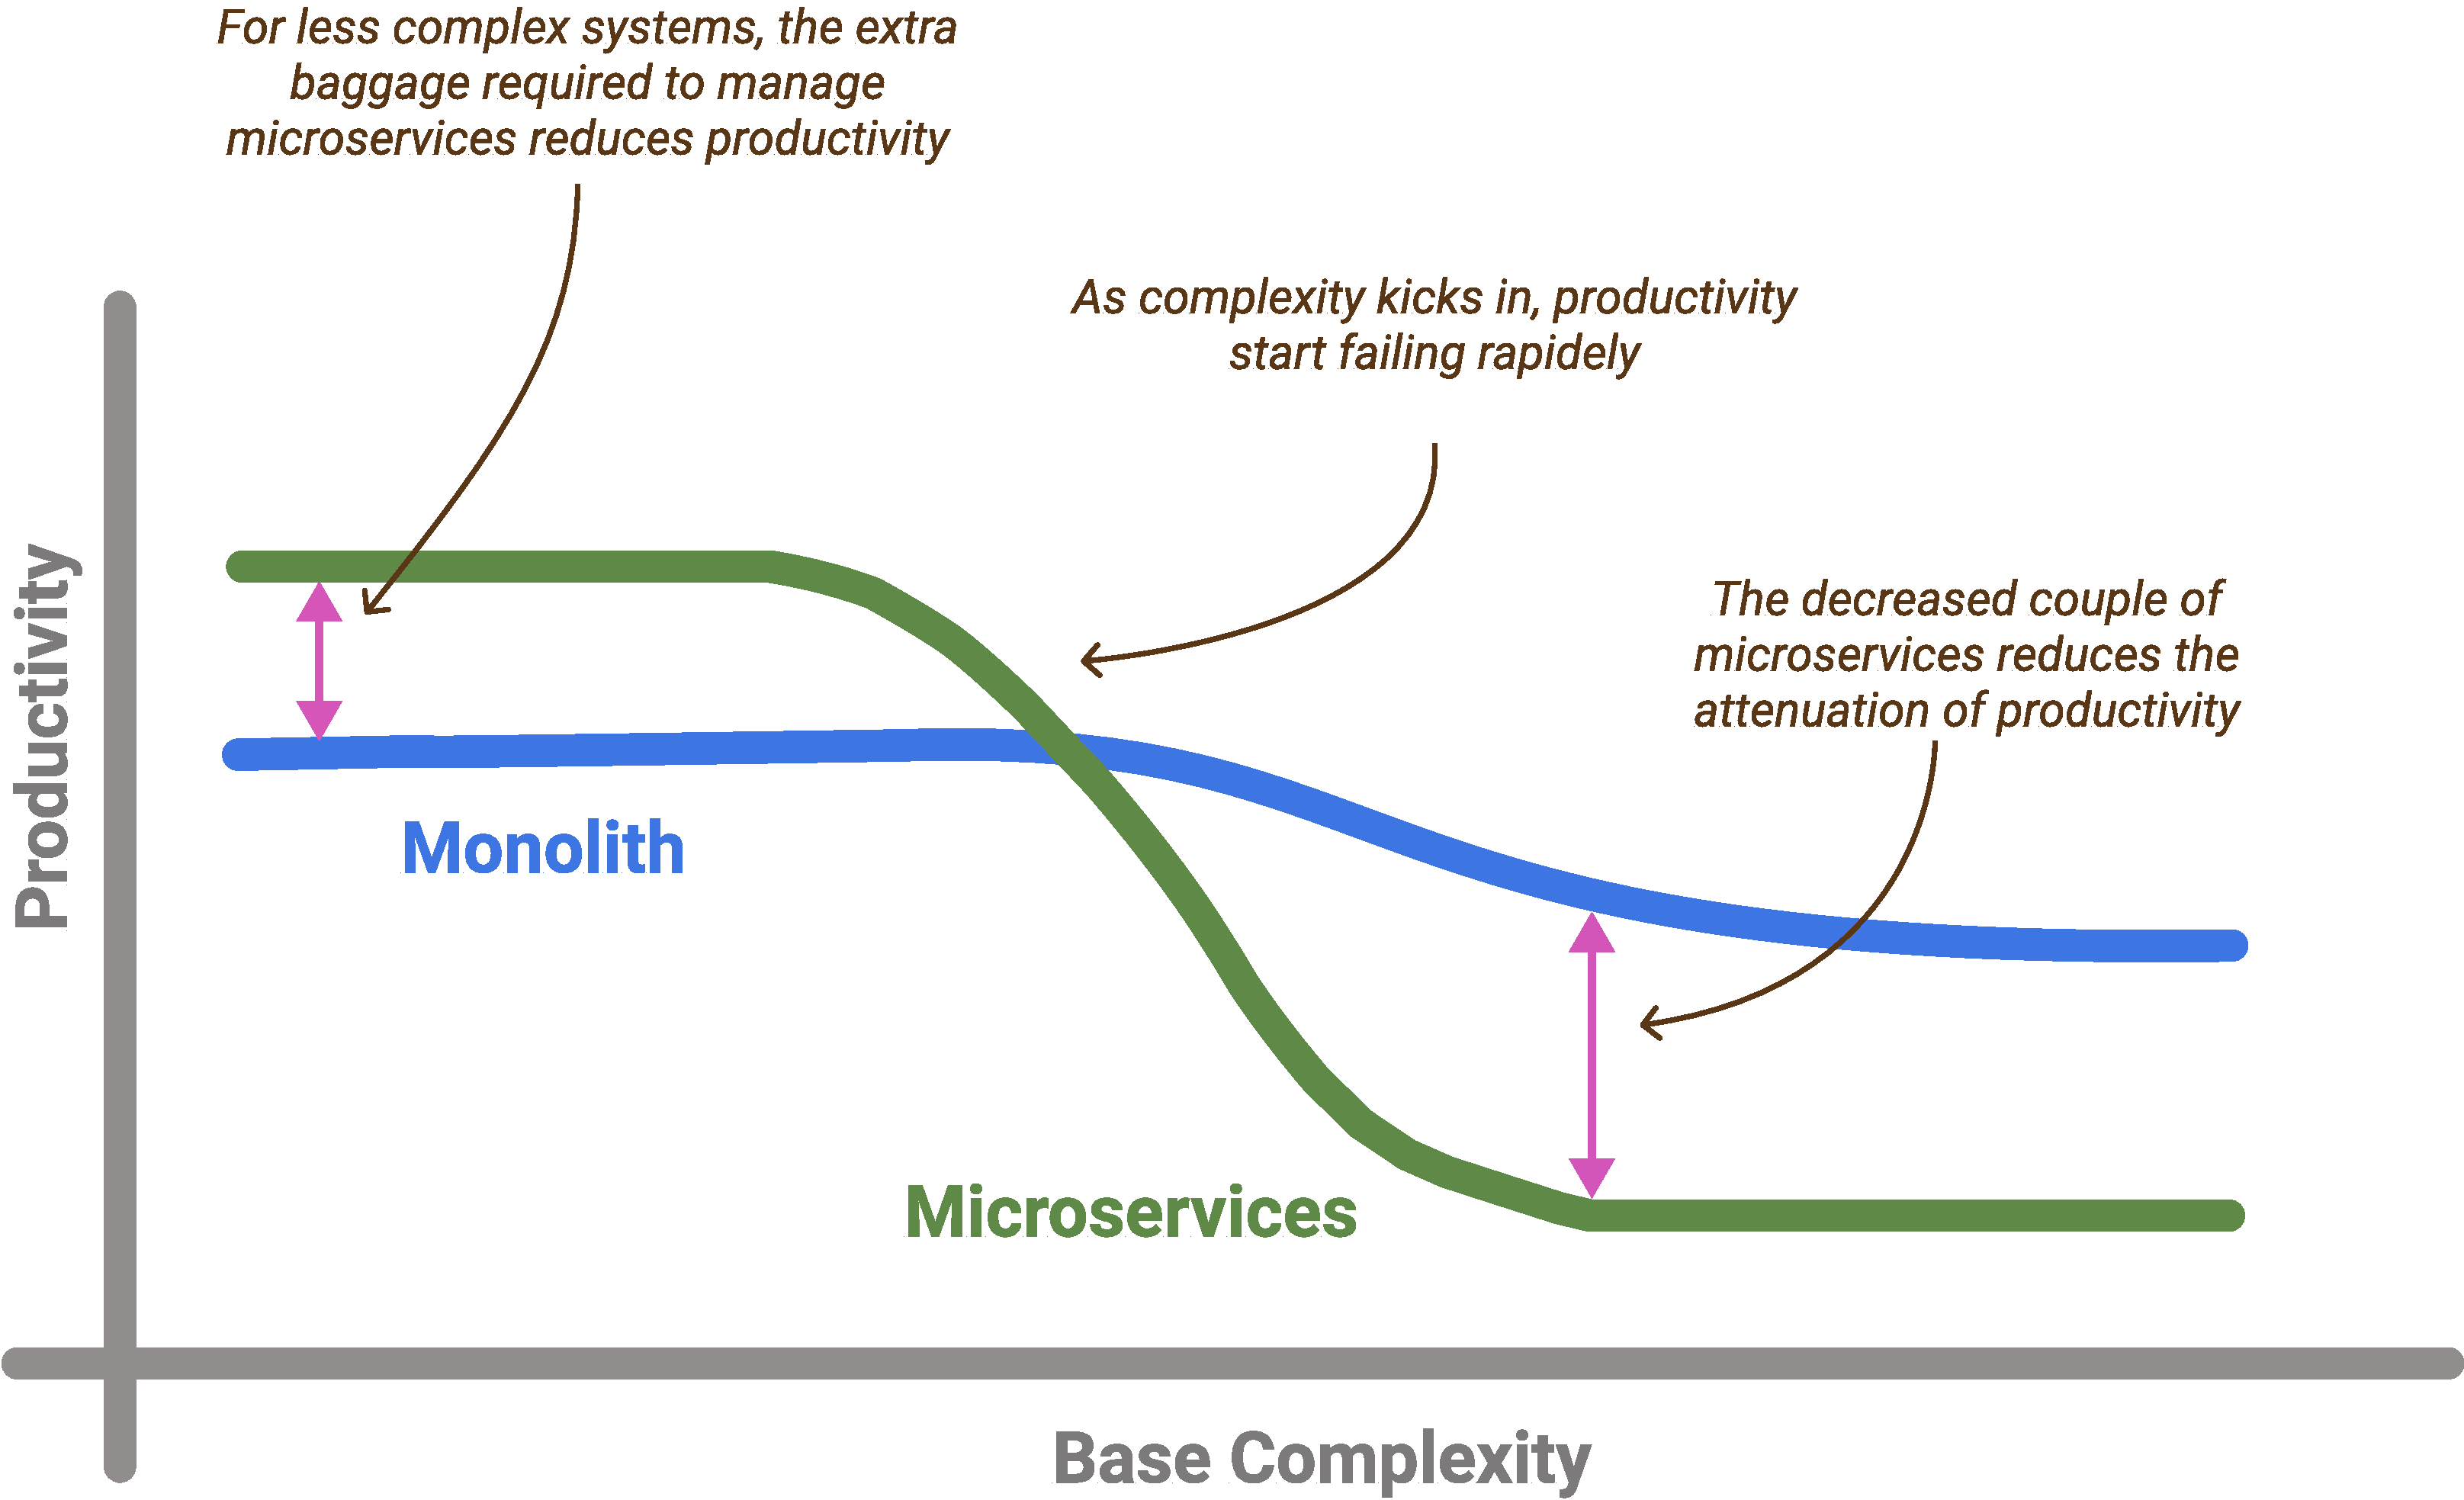
\includegraphics[width=1\textwidth]{Pictures/Monolith_vs_Microservice.pdf}
    \caption{Relation between system complexity and architectures. Source: https://martinfowler.com/bliki/MicroservicePremium.html}
    \label{fig:monolith_vs_microservice}
\end{figure}

\subsection{Initial concept diagram and discussion}\label{subsec:initial-concept-diagram}
\begin{figure}[H]
    \centering
    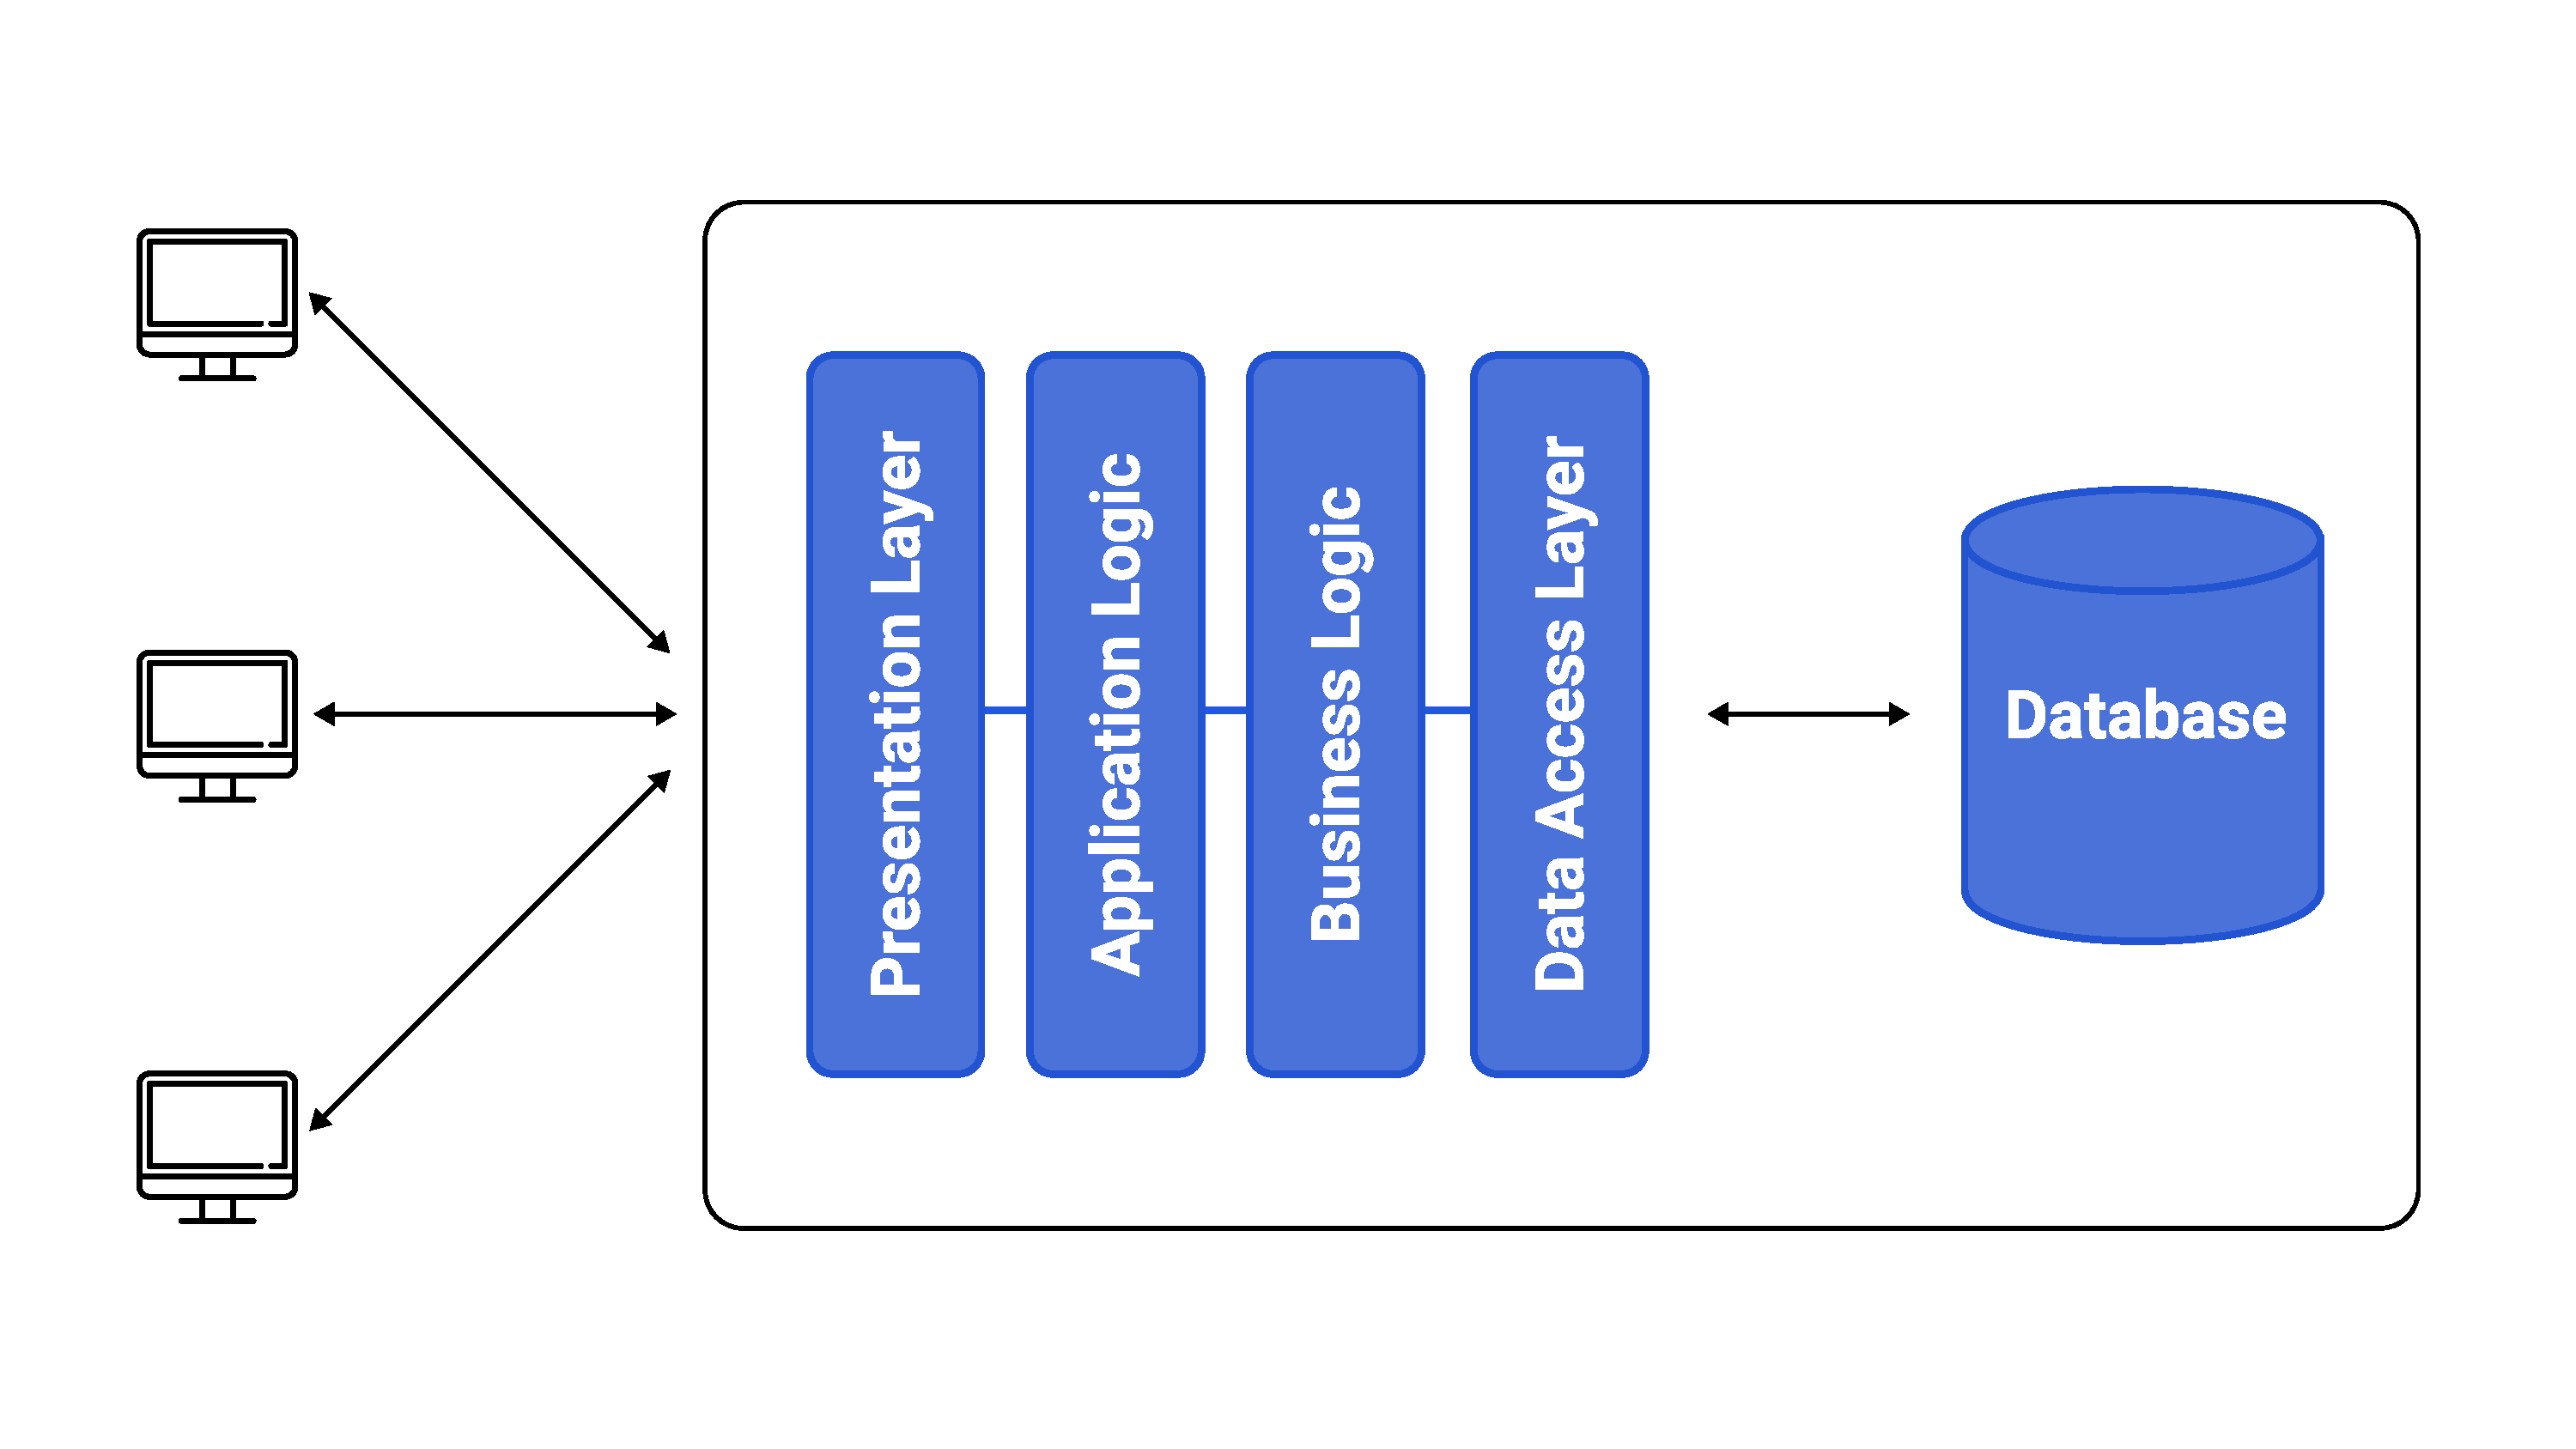
\includegraphics[width=1\textwidth]{Pictures/Monolith_architecture.pdf}
    \caption{Monolithic architecture diagram. Source: }\label{fig:figure2}
\end{figure}

\subsection{Application layers}\label{subsec:application-layers}
\begin{itemize}
    \item \textbf{Presentation Layer.} Responsible for external communication, e.g.\ API gateway, front-end application etc.
    \item \textbf{Application Logic.} Responsible for interaction with user, for instance email sender, realtime notification service etc.
    \item \textbf{Business Logic.} Keeps application business logics, request handlers etc.
    \item \textbf{Data Access Layer.} Interface of interaction with database.
    \item \textbf{Database.} Simply, database itself.\ For instance, Relational, NoSQL, Cache database etc.
\end{itemize}

\subsection{Monolith Architecture: Cons and Props}\label{subsec:monolith-architecture:-cons-and-props}

A monolith is built as a large system with a single code base and deployed as a single unit, usually behind a load balancer.
It typically consists of four major components: a user interface, business logic, a data interface and a database.
Monoliths offer several advantages, particularly when it comes to operational overhead requirements.
Here are some of those basic benefits:

\begin{itemize}
    \item \textbf{Simplicity.} Monolithic architectures are simple to build, test and deploy.
    These apps can scale horizontally, in one direction, by running several copies of the application behind a load balancer.
    Cross-cutting concerns: With a single codebase, monolithic apps can easily handle cross-cutting concerns, such as logging,
    configuration management and performance monitoring.
    Another advantage associated with the simplicity of monolithic apps is easier deployment.
    When it comes to monolithic applications, you do not have to handle many deployments – just one file or directory.
    \item \textbf{Performance.} Components in a monolith typically share memory which is faster than service-to-service communications using
    IPC [INSERTREF] or other mechanisms.
    \item \textbf{Easier debugging and testing.}
    In contrast to the microservices architecture, monolithic applications are much easier to debug and test.
    Since a monolithic app is a single indivisible unit, you can run end-to-end testing much faster.
    \item \textbf{Easier development.} As long as the monolithic approach is a standard way of building applications,
    any engineering team has the right knowledge and capabilities to develop a monolithic application.
\end{itemize}
But one major drawback of monolithic architectures is tight coupling.
Over time, monolithic components become tightly coupled and entangled.
This coupling effects management, scalability and continuous deployment.
Other cons that stem from tight coupling include:

\begin{itemize}
    \item \textbf{Understanding.} When a monolithic application scales up, it becomes too complicated to understand.
    Also, a complex system of code within one application is hard to manage.
    \item \textbf{Reliability.} An error in any of the modules in the application can bring the entire application down.
    \item \textbf{Updates.} Due to a single large codebase and tight coupling, the entire application would have to deploy
    for each update.
    \item \textbf{Technology stack.} A monolithic application must use the same technology stack throughout.
    Changes to the technology stack are expensive, both in terms of the time and cost involved.
    \item \textbf{Scalability.} You cannot scale components independently, only the whole application.
\end{itemize}

\subsection{Decoupling Monolith using CQRS}\label{subsec:decoupling-monolith-using-cqrs}
Answer the questions:
\begin{itemize}
    \item What is CQRS?
    \item Why do we use CQRS?
    \item How CQRS helps us to decouple monolith?
\end{itemize}
\begin{figure}[H]
    \centering
    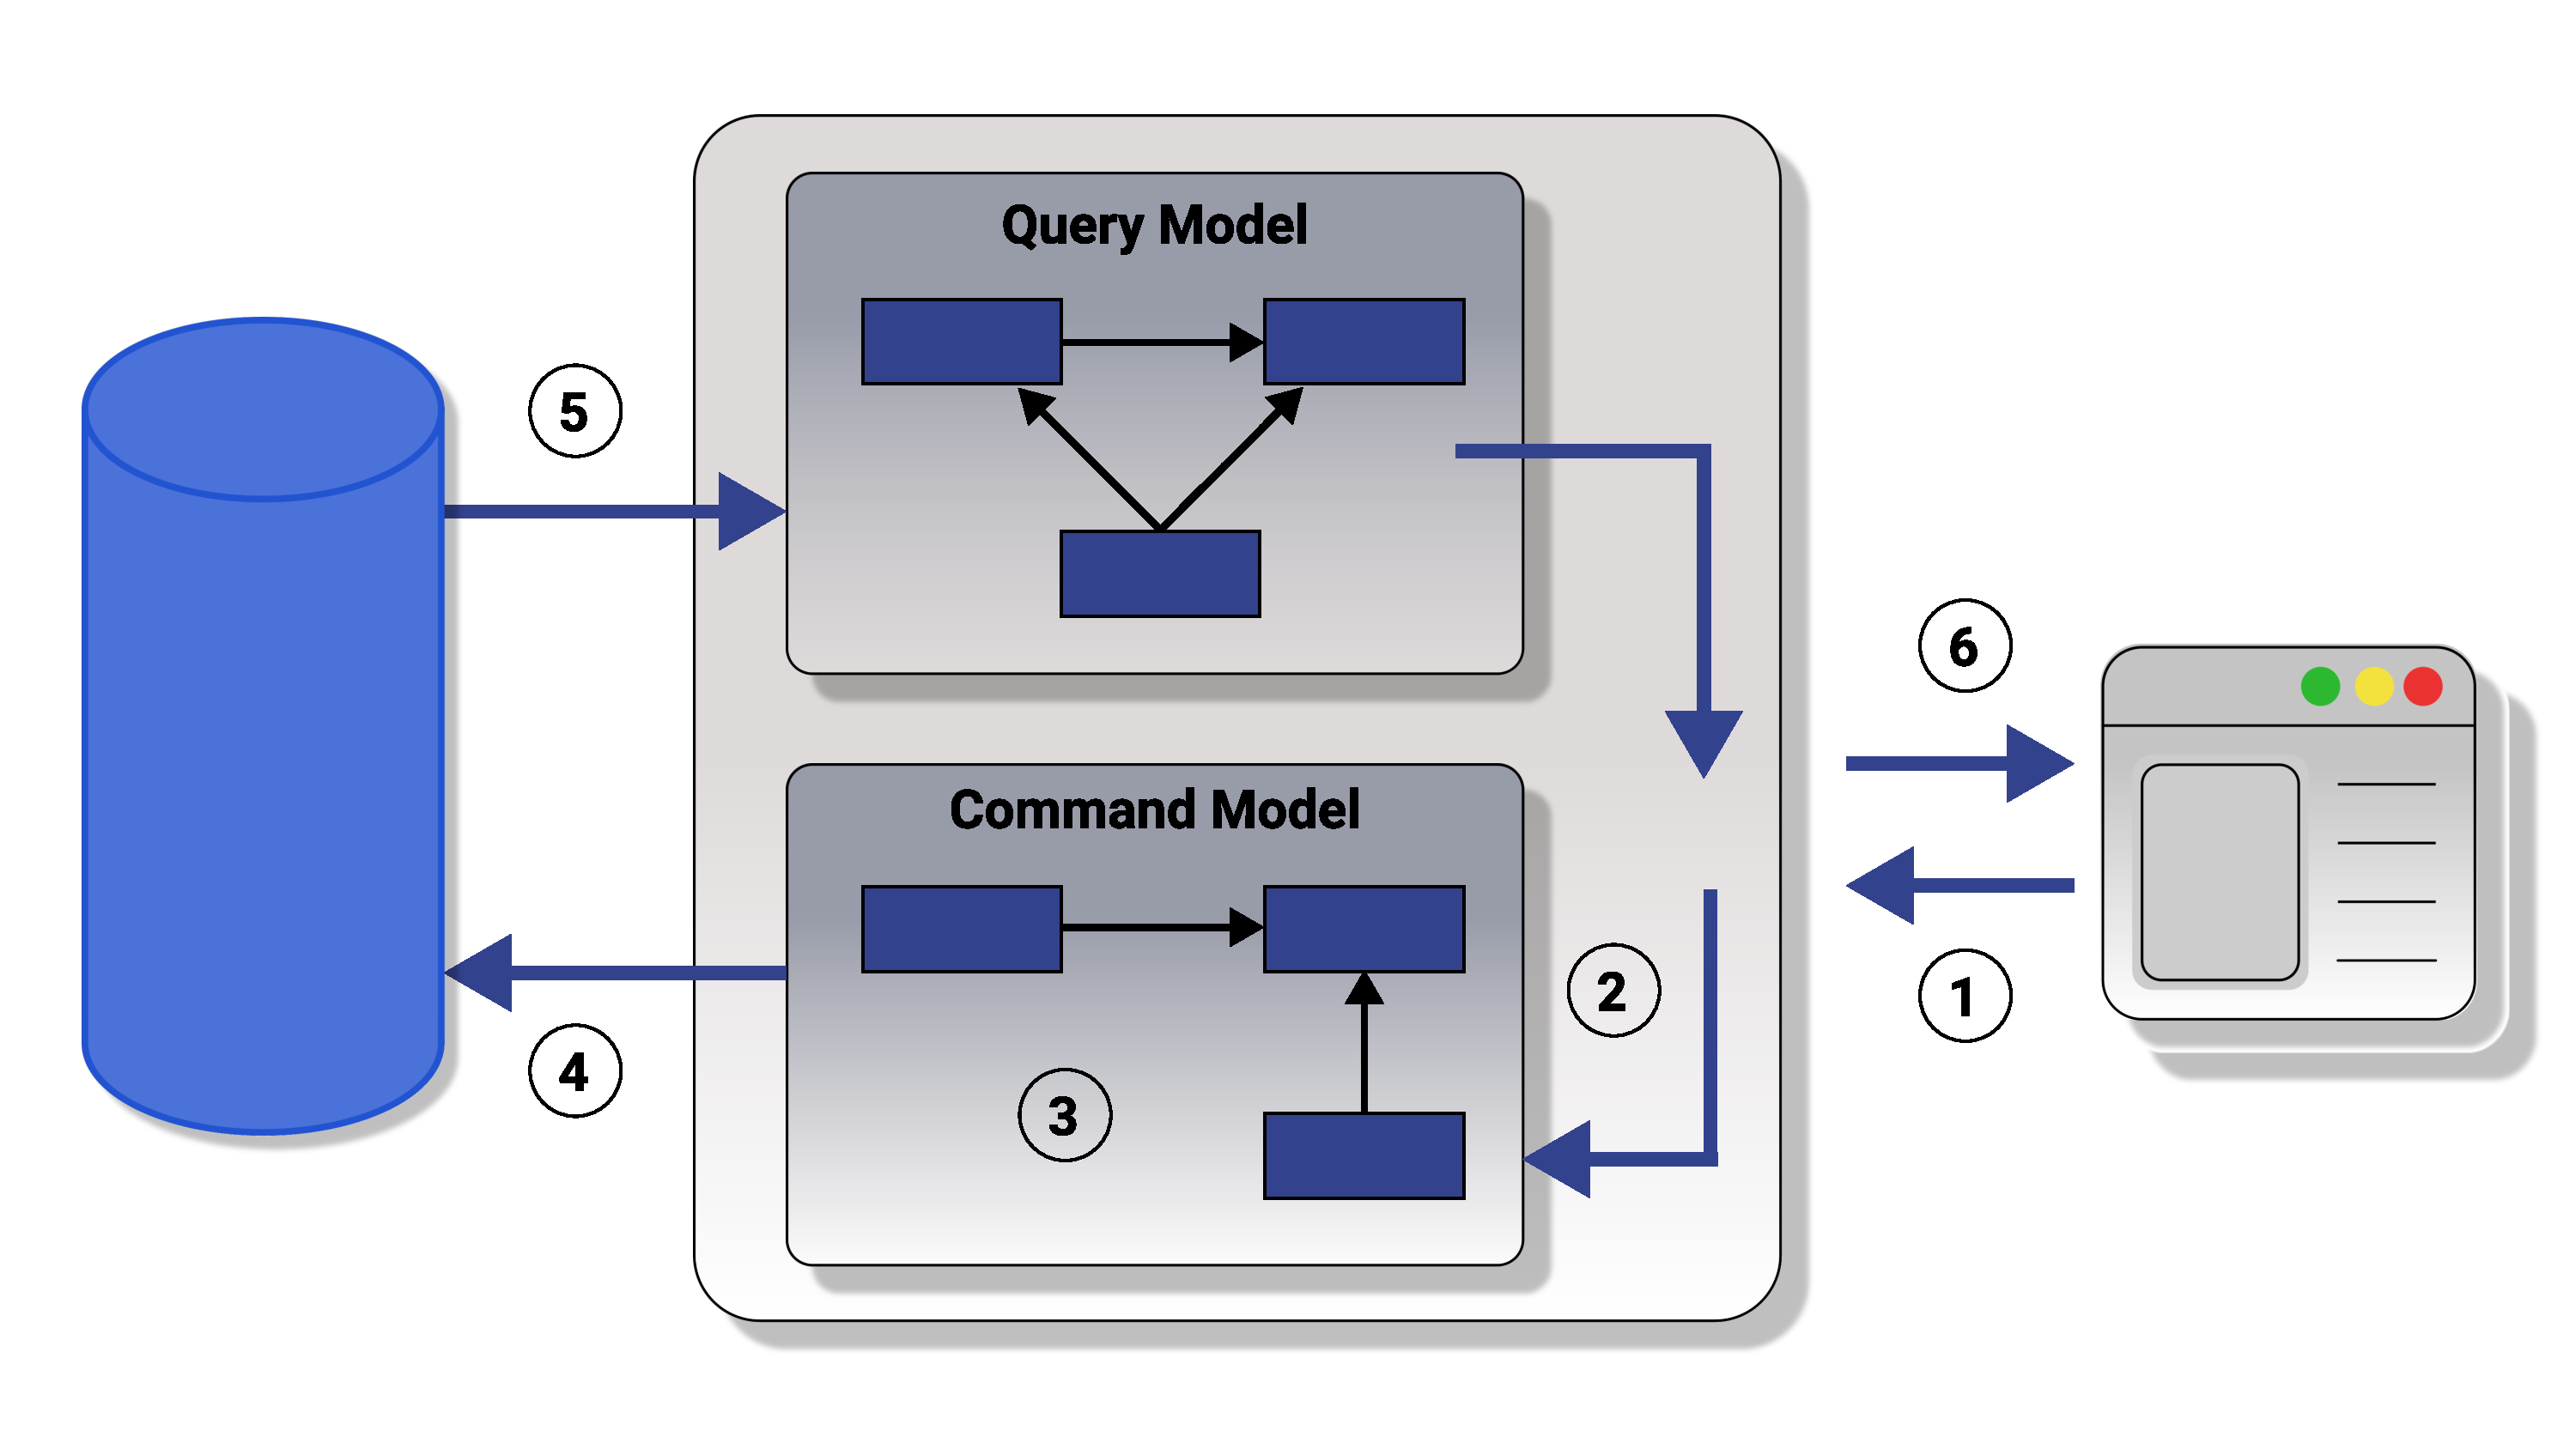
\includegraphics[width=1\textwidth]{Pictures/cqrs.pdf}
    \caption{CQRS Conceptual diagram. Source: https://martinfowler.com/bliki/CQRS.html}\label{fig:figure}
\end{figure}

\subsection{Discussion on JWT Authentication}\label{subsec:discussion-on-jwt-authentication}
\begin{figure}[H]
    \centering
    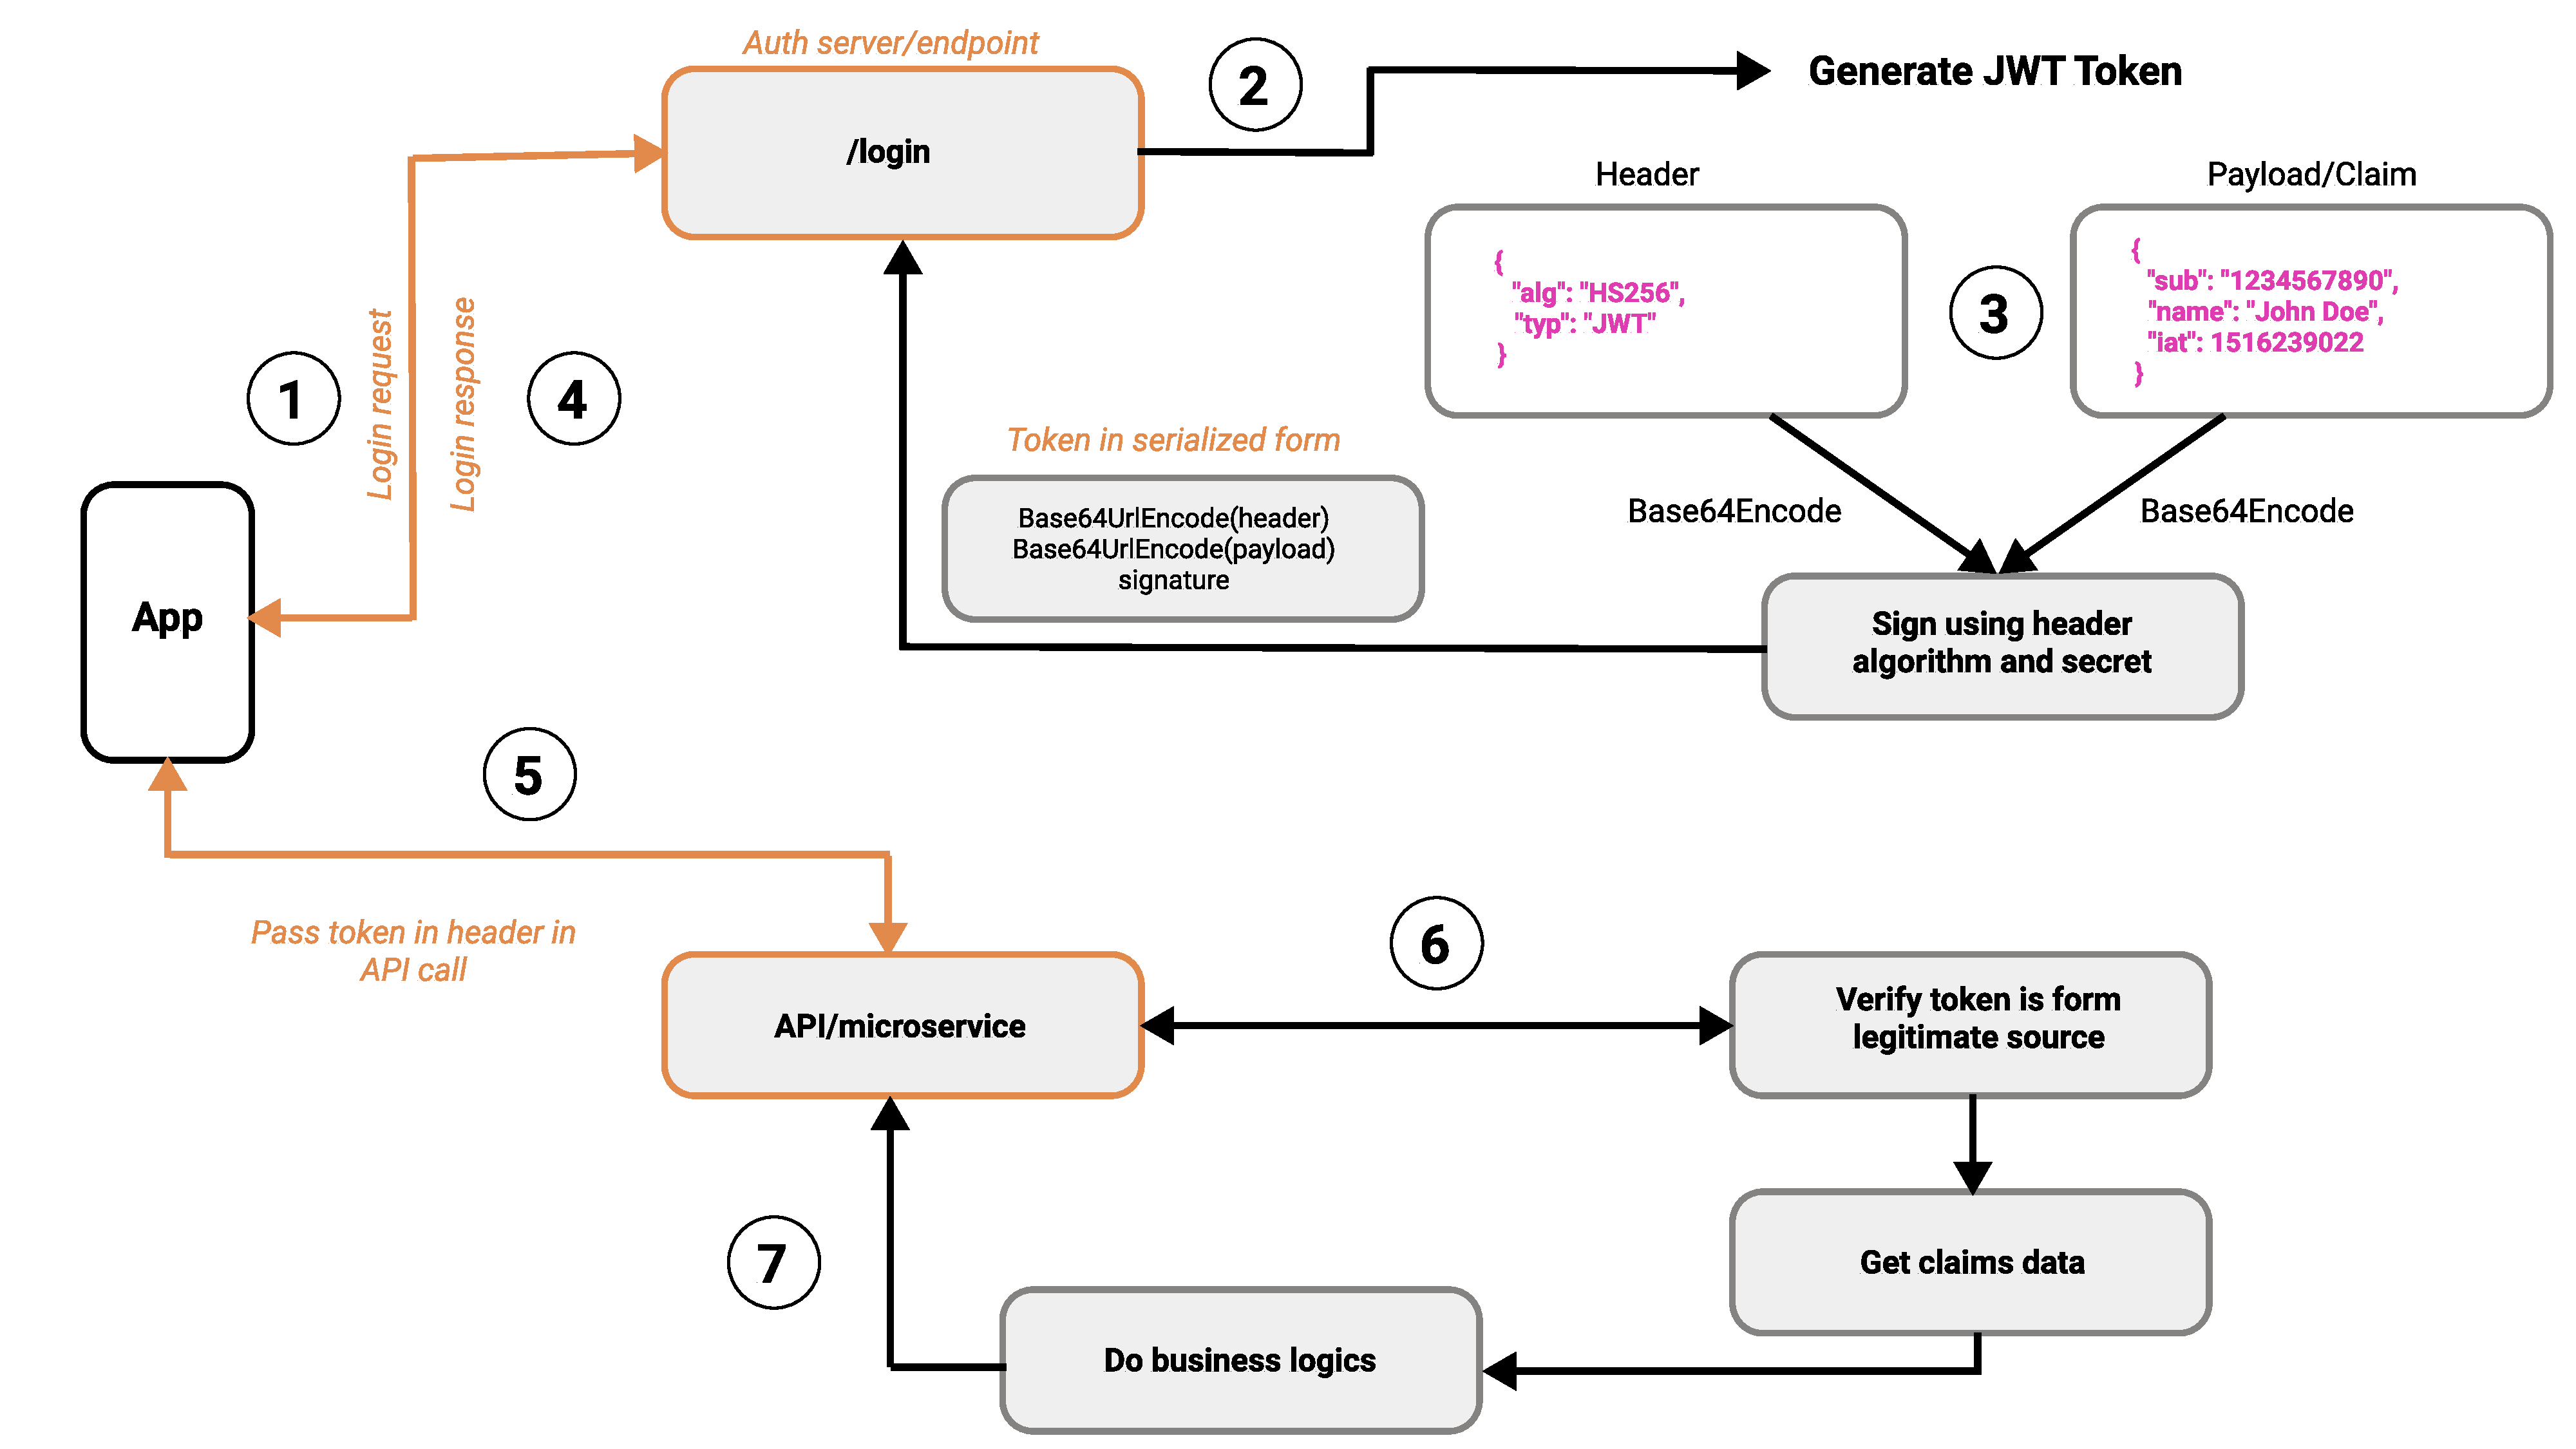
\includegraphics[width=1\textwidth]{Pictures/jwt_auth_scheme.pdf}
    \caption{CQRS Conceptual diagram. Source: https://martinfowler.com/bliki/CQRS.html}\label{fig:figure3}
\end{figure}

\subsection{Planned technologies}\label{subsec:planned-technologies}
\begin{itemize}
    \item \textbf{SDK}: \href{https://dotnet.microsoft.com/download/dotnet/5.0}{.NET Core 5.0}
    \item \textbf{DBMS}: \href{https://www.postgresql.org/}{PostgreSQL 13}
    \item \textbf{CI}: \href{https://docs.github.com/en/actions}{GitHub Actions}
    \item \textbf{ORM}: \href{https://www.nuget.org/packages/Microsoft.EntityFrameworkCore/5.0.7?_src=template}{Entity Framework Core 5.0.7}
    \item \textbf{EF Core For PostgreSQL Provider}: \href{https://www.nuget.org/packages/Npgsql.EntityFrameworkCore.PostgreSQL/5.0.7?_src=template}{Npgsql.EntityFrameworkCore.PostgreSQL 5.0.7}
    \item \textbf{Mediator Pattern Library} \href{https://www.nuget.org/packages/MediatR/9.0.0?_src=template}{MediatR 9.0.0}
    \item \textbf{Validation Library}: \href{https://www.nuget.org/packages/FluentValidation/10.2.3?_src=template}{Fluent Validation}
    \item \textbf{JWT Library}: \href{https://www.nuget.org/packages/System.IdentityModel.Tokens.Jwt}{System JWT 6.8.0}
    \item \textbf{JWT Auxiliary Library}: \href{https://www.nuget.org/packages/System.IdentityModel.Tokens}{System Tokens 6.11.1}
    \item \textbf{JWT Bearer}: \href{https://www.nuget.org/packages/Microsoft.AspNetCore.Authentication.JwtBearer/5.0.7?_src=template}{Microsoft Jwt Bearer}
    \item \textbf{Swagger Library}: \href{https://www.nuget.org/packages/Swashbuckle.AspNetCore/5.6.3?_src=template}{Swashbuckle 6.1.4}
\end{itemize}


\section{Security aspects of HTTPS protocol}\label{sec:security-aspects-of-https-protocol}
General discussion on HTTP here.

\subsection{Diffie-Hellman Protocol}\label{subsec:diffie-hellman-protocol}

Diffie–Hellman key exchange [INSERTREF] is a method of securely exchanging cryptographic keys over a public channel
and was one of the first public-key protocols
as conceived by Ralph Merkle and named after Whitefield Diffie and Martin Hellman.
DH is one of the earliest practical examples of public key exchange implemented within the field of cryptography.

Published in 1976 by Diffie and Hellman, this is the earliest publicly known work that proposed the idea of a private
key and a corresponding public key.

Traditionally, secure encrypted communication between two parties required that they first exchange keys by some secure physical means,
such as paper key lists transported by a trusted courier.
The Diffie–Hellman key exchange method allows two parties that have no prior knowledge of
each other to jointly establish a shared secret key over an insecure channel.
This key can then be used to encrypt subsequent communications using a symmetric-key cipher.

Although Diffie–Hellman key agreement itself is a non-authenticated key-agreement protocol, it provides the basis for a
variety of authenticated protocols,
and is used to provide forward secrecy in Transport Layer Security's ephemeral modes
(referred to as EDH or DHE depending on the cipher suite).

\textbf{Description}:

Diffie–Hellman key exchange establishes a shared secret between two parties that can be used for secret communication
for exchanging data over a public network.
An analogy illustrates the concept of public key exchange by using colors instead of very large numbers:

\begin{figure}[H]
    \centering
    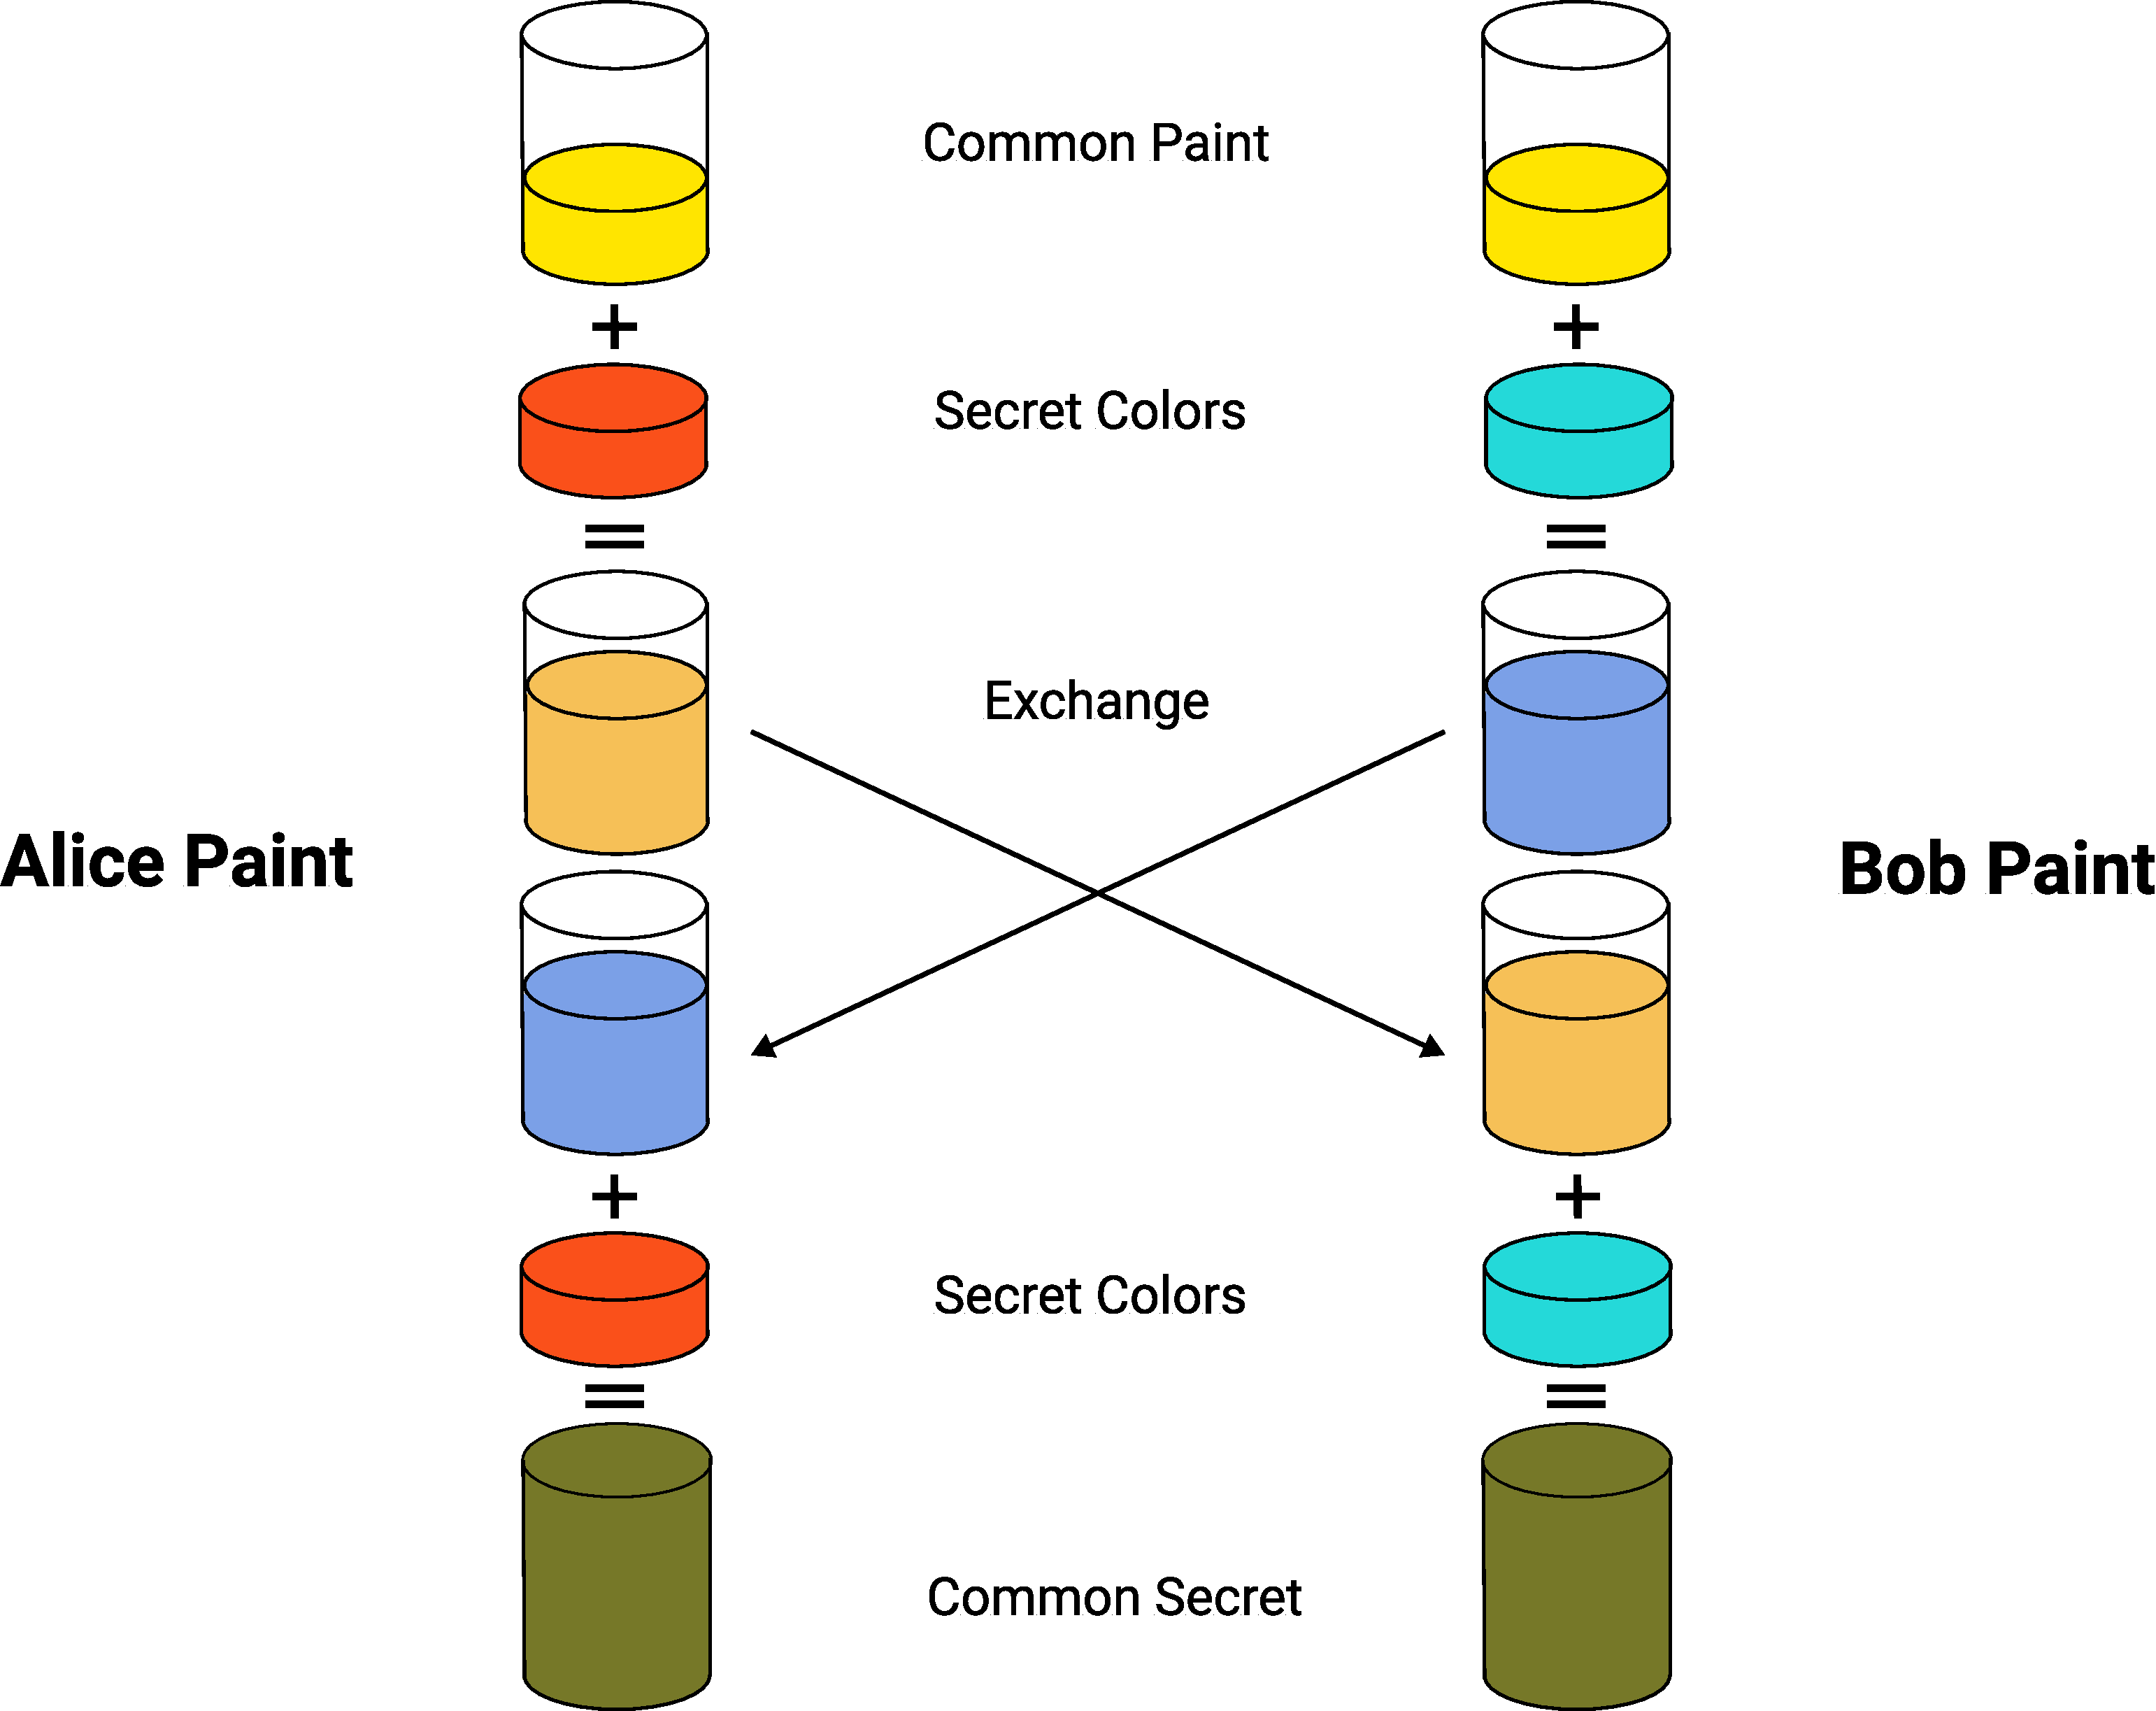
\includegraphics[width=1\textwidth]{Pictures/Diffie-Hellman.pdf}
    \caption{Illustration of the concept behind Diffie–Hellman key exchange}\label{fig:figure4}
\end{figure}

The process begins by having the two parties, Alice and Bob, publicly agree on an arbitrary starting color that does
not need to be kept secret (but should be different every time).
In this example, the color is yellow.
Each person also selects a secret color that they keep to themselves – in this case, red and blue-green.
The crucial part of the process is that Alice and Bob each mix their own secret color together with their mutually
shared color, resulting in orange-tan and light-blue mixtures respectively, and then publicly exchange the two mixed colors.
Finally, each of them mixes the color they received from the partner with their own private color.
The result is a final color mixture (yellow-brown in this case) that is identical to the partner's final color mixture.

If a third party listened to the exchange, it would only know the common color (yellow) and the first mixed colors
(orange-tan and light-blue), but it would be difficult for this party to determine the final secret color (yellow-brown).
Bringing the analogy back to a real-life exchange using large numbers rather than colors, this determination is
computationally expensive.
It is impossible to compute in a practical amount of time even for modern supercomputers.

\textbf{Cryptographic explanation}:
\newline
The simplest and the original implementation of the protocol uses the multiplicative group of integers modulo p,
where p is prime, and g is a primitive root modulo p.
These two values are chosen in this way to ensure that the resulting shared secret can take on any value from 1 to p–1.
Here is an example of the protocol, with non-secret values in \textcolor{blue}{blue}, and secret values in \textcolor{red}{red}.
\newline
\begin{enumerate}
    \item Alice and Bob publicly agree to use a modulus \textcolor{blue}{p = 23} and base \textcolor{blue}{g = 5} (which is a primitive root modulo 23).

    \item Alice chooses a secret integer $\textcolor{red}{a} = 4$, then sends Bob $\textcolor{blue}{A} = \textcolor{blue}{g}^{\textcolor{red}{a}} \, mod  \, \textcolor{blue}{p}$
    \begin{itemize}
        \item $\textcolor{blue}{A} = \textcolor{blue}{5}^{\textcolor{red}{4}} \, mod  \, \textcolor{blue}{23} = \textcolor{blue}{4}$
    \end{itemize}

    \item Bob chooses a secret integer $\textcolor{red}{b} = 3$, then sends Alice $\textcolor{blue}{B} = \textcolor{blue}{g}^{\textcolor{red}{b}} \, mod  \, \textcolor{blue}{p}$
    \begin{itemize}
        \item $\textcolor{blue}{B} = \textcolor{blue}{5}^{\textcolor{red}{3}} \, mod  \, \textcolor{blue}{23} = \textcolor{blue}{10}$
    \end{itemize}

    \item Alice computes $\textcolor{red}{s} = \textcolor{blue}{B}^{\textcolor{red}{a}} \, mod \, p$
    \begin{itemize}
        \item $\textcolor{red}{s} = \textcolor{blue}{10}^{\textcolor{red}{4}} \, mod \, \textcolor{blue}{23} = \textcolor{red}{18}$
    \end{itemize}

    \item Bob computes $\textcolor{red}{s} = \textcolor{blue}{A}^{\textcolor{red}{b}} \, mod \, p$
    \begin{itemize}
        \item $\textcolor{red}{s} = \textcolor{blue}{4}^{\textcolor{red}{3}} \, mod \, \textcolor{blue}{23} = \textcolor{red}{18}$
    \end{itemize}

    \item Alice and Bob now share a secret (the number 18).
\end{enumerate}

Both Alice and Bob have arrived at the same values because under mod p:
\newline
\newline
$\textcolor{blue}{A}^{\textcolor{red}{b}} \, mod \, \textcolor{blue}{p} = \textcolor{blue}{g}^{\textcolor{red}{ab}} \, mod \, \textcolor{blue}{p} = \textcolor{blue}{g}^{\textcolor{red}{ba}} \, mod \, \textcolor{blue}{p} = \textcolor{blue}{B}^{\textcolor{red}{a}} \, mod \, \textcolor{blue}{p}$
\newline
More specifically:
\newline
\newline
$(\textcolor{blue}{g}^{\textcolor{red}{a}} \, mod \, \textcolor{blue}{p})^{\textcolor{red}{b}} \, mod \, \textcolor{blue}{p} = (\textcolor{blue}{g}^{\textcolor{red}{b}} \, mod \, \textcolor{blue}{p})^{\textcolor{red}{a}}$
\newline

Only a and b are kept secret.
All the other values – p, g, ga mod p, and gb mod p – are sent in the clear.
The strength of the scheme comes from the fact that gab mod p = gba mod p take extremely long times to compute by any
known algorithm just from the knowledge of p, g, ga mod p, and gb mod p.
Once Alice and Bob compute the shared secret they can use it as an encryption key, known only to them, for sending
messages across the same open communications channel.

Of course, much larger values of a, b, and p would be needed to make this example secure, since there are only 23 possible
results of n mod 23.
However, if p is a prime of at least 600 digits, then even the fastest modern computers using the fastest known algorithm
cannot find a given only g, p and ga mod p.
Such a problem is called the discrete logarithm problem [INSERTREF].
The computation of ga mod p is known as modular exponentiation and can be done efficiently even for large numbers.
Note that g need not be large at all, and in practice is usually a small integer (like 2, 3, ...).
\newline
\textbf{Secrecy Chart}:
\newline
The chart below depicts who knows what, again with non-secret values in \textcolor{blue}{blue}, and secret values in \textcolor{red}{red}.
Here Eve is an eavesdropper – she watches what is sent between Alice and Bob, but she does not alter the contents of their communications.

\begin{itemize}
    \item \textcolor{blue}{g} = public (prime) base, known to Alice, Bob, and Eve. $\textcolor{blue}{g = 5}$
    \item \textcolor{blue}{p} = public (prime) modulus, known to Alice, Bob, and Eve. $\textcolor{blue}{p = 23}$
    \item \textcolor{red}{a} = Alice's private key, known only to Alice. $\textcolor{red}{a = 6}$
    \item \textcolor{red}{b} = Bob's private key known only to Bob. $\textcolor{red}{b = 15}$
    \item \textcolor{blue}{A} = Alice's public key, known to Alice, Bob, and Eve. $\textcolor{blue}{A = g}^{\textcolor{red}{a}} \, mod \, \textcolor{blue}{p = 8}$
    \item \textcolor{blue}{B} = Bob's public key, known to Alice, Bob, and Eve. $\textcolor{blue}{B = g}^{\textcolor{red}{a}} \, mod \, \textcolor{blue}{p = 8}$
\end{itemize}

\pagebreak
\begin{center}
    \begin{table}
        \begin{tabular}{|c|c|c|c|c|c|}
            \hline
            \multicolumn{2}{|c|}{Alice} & \multicolumn{2}{c|}{Bob} & \multicolumn{2}{c|}{Eve}
            \cr \hline
            known & unknown & known & unknown & known & unknown
            \cr \hline
            $\textcolor{blue}{p = 23}$ & & $\textcolor{blue}{p = 23}$  & & $\textcolor{blue}{p = 23}$ &
            \cr \hline
            $\textcolor{blue}{g = 5}$ & & $\textcolor{blue}{g = 5}$ & & $\textcolor{blue}{g = 5}$ &
            \cr \hline
            $\textcolor{red}{a = 6}$ & $\textcolor{red}{b}$ & $\textcolor{red}{b = 15}$ & $\textcolor{red}{a}$ & & $\textcolor{red}{a, b}$
            \cr \hline
            $\textcolor{blue}{A = 5}^{\textcolor{red}{a}} \, mod \, \textcolor{blue}{23}$ & & $\textcolor{blue}{B = 5}^{\textcolor{red}{b}} \, mod \, \textcolor{blue}{23}$ & & &
            \cr \hline
            $\textcolor{blue}{A = 5}^{\textcolor{red}{6}} \, mod \, \textcolor{blue}{23} = \textcolor{blue}{8}$ & & $\textcolor{blue}{B = 5}^{\textcolor{red}{15}} \, mod \, \textcolor{blue}{23} = \textcolor{blue}{19}$ & & &
            \cr \hline
            $\textbf{\textcolor{blue}{B}} = \textbf{\textcolor{blue}{19}}$ & & $\textbf{\textcolor{blue}{A}} = \textbf{\textcolor{blue}{8}}$ & & $\textcolor{blue}{A} = \textcolor{blue}{8}$, $\textcolor{blue}{B} = \textcolor{blue}{19}$ &
            \cr \hline
            $\textbf{\textcolor{red}{s}} = \textcolor{blue}{B}^{\textcolor{red}{a}} \, mod \, \textcolor{blue}{23}$ & & $\textbf{\textcolor{red}{s}} = \textcolor{blue}{A}^{\textcolor{red}{b}} \, mod \, \textcolor{blue}{23}$ & & &
            \cr \hline
            $\textbf{\textcolor{red}{s}} = \textcolor{blue}{19}^{\textcolor{red}{6}} \, mod \, \textcolor{blue}{23} = \textcolor{red}{2}$ & & $\textbf{\textcolor{red}{s}} = \textcolor{blue}{A}^{\textcolor{red}{b}} \, mod \, \textcolor{blue}{23} = \textcolor{red}{2}$ & & &
            \cr \hline

        \end{tabular}
        \label{tab:table}
    \end{table}
\end{center}

Now \textcolor{red}{s} is the shared secret key and it is known to both Alice and Bob, but not to Eve.
Note that it is not helpful for Eve to compute \textcolor{blue}{AB}, which equals
$\textcolor{blue}{g}^{\textcolor{red}{a} + \textcolor{red}{b}} \, mod \, \textcolor{blue}{p}$.

Note: It should be difficult for Alice to solve for Bob's private key or for Bob to solve for Alice's private key.
If it is not difficult for Alice to solve for Bob's private key (or vice versa), Eve may simply substitute her own
private / public key pair, plug Bob's public key into her private key, produce a fake shared secret key, and solve for
Bob's private key (and use that to solve for the shared secret key.
Eve may attempt to choose a public / private key pair that will make it easy for her to solve for Bob's private key).
    \chapter{Mango Messenger}\label{ch:mango-messenger}


\section{Web API Documentation}\label{sec:web-api-documentation}

\subsection{Auth}\label{subsec:auth}
\begin{itemize}
        %% Register Endpoint
    \item \textbf{Endpoint}: /api/auth/register
    \begin{itemize}
        \item \textbf{Description}: Registers user in a messenger
        \item \textbf{Request type}: POST
        \item \textbf{Request body}:
        \begin{spverbatim}
        {
            "phoneNumber": "string",
            "email": "string",
            "displayName": "string",
            "password": "string",
            "verificationMethod": number,
            "termsAccepted": boolean
        }
        \end{spverbatim}
        \item  \textbf{Response example}:

        \textbf{200 Success}:

        \begin{spverbatim}
        {
            "message": "SUCCESS",
            "success": true
        }
        \end{spverbatim}

        \textbf{400 Bad Request}:

        \begin{spverbatim}
        {
            "errorMessage": "string",
            "errorDetails": "string",
            "statusCode": 0,
            "success": true
        }
        \end{spverbatim}

        \textbf{409 Conflict}:

        \begin{spverbatim}
        {
            "errorMessage": "string",
            "errorDetails": "string",
            "statusCode": 0,
            "success": true
        }
        \end{spverbatim}
        \item \textbf{Response messages}:
        \begin{enumerate}
            \item Success.
            \item User already registered.
            \item Weak password.
            \item Invalid email.
            \item Invalid verification method.
            \item Invalid display name.
            \item Phone occupied.
        \end{enumerate}
    \end{itemize}
    %% Register Endpoint

    %% Verify Email Endpoint
    \item \textbf{Endpoint}: api/auth/verify-email

    \begin{itemize}
        \item \textbf{Description}: Sends verification request.
        User receives confirmation link via email.
        \item \textbf{Request type}: GET
        \begin{spverbatim}
        {
            "email": "string",
            "userId": "string"
        }
        \end{spverbatim}
        \item  \textbf{Response example}:

        \textbf{200 Success}:

        \begin{spverbatim}
        {
            "message": "SUCCESS",
            "success": true
        }
        \end{spverbatim}

        \textbf{400 Bad Request}:

        \begin{spverbatim}
        {
            "errorMessage": "string",
            "errorDetails": "string",
            "statusCode": 0,
            "success": false
        }
        \end{spverbatim}

        \textbf{409 Conflict}:

        \begin{spverbatim}
        {
            "errorMessage": "string",
            "errorDetails": "string",
            "statusCode": 0,
            "success": false
        }
        \end{spverbatim}
        \item \textbf{Response messages}:
        \begin{enumerate}
            \item Success.
            \item User already registered.
            \item Weak password.
            \item Invalid email.
            \item Invalid verification method.
            \item Invalid display name.
            \item Phone occupied.
        \end{enumerate}
        \item \textbf{Response messages}:
        \begin{enumerate}
            \item Success.
            \item Invalid user id.
            \item Email already verified.
        \end{enumerate}
    \end{itemize}
    %% Verify Email Endpoint

    %% Verify Phone Endpoint
    \item \textbf{Endpoint}: api/auth/verify-phone
    \begin{itemize}
        \item \textbf{Description}: Sends SMS to user phone.
        \item \textbf{Request type}: POST
        \item \textbf{Request body}:
        \begin{spverbatim}
        {
            "confirmationCode": 0,
            "userId": "string"
        }
        \end{spverbatim}
        \item  \textbf{Response example}:

        \textbf{200 Success}:

        \begin{spverbatim}
        {
            "message": "SUCCESS",
            "success": true
        }
        \end{spverbatim}

        \textbf{400 Bad Request}:

        \begin{spverbatim}
        {
            "errorMessage": "string",
            "errorDetails": "string",
            "statusCode": 0,
            "success": false
        }
        \end{spverbatim}

        \textbf{409 Conflict}:

        \begin{spverbatim}
        {
            "errorMessage": "string",
            "errorDetails": "string",
            "statusCode": 0,
            "success": false
        }
        \end{spverbatim}
        \item \textbf{Response messages}:
        \begin{enumerate}
            \item Success.
            \item Invalid or expired.
            \item Phone already verified
        \end{enumerate}
    \end{itemize}
    %% Verify Phone Endpoint

    %% Login Endpoint
    \item \textbf{Endpoint}: api/auth/login

    \begin{itemize}
        \item \textbf{Description}: Performs login to the messenger.
        \item \textbf{Request type}: POST
        \item \textbf{Request body}:
        \begin{spverbatim}
        {
            "email": "string",
            "password": "string"
        }
        \end{spverbatim}
        \item  \textbf{Response example}:

        \textbf{200 Success}:

        \begin{spverbatim}
        {
            "refreshTokenId": "string",
            "accessToken": "string",
            "message": "string",
            "success": true
        }
        \end{spverbatim}

        \textbf{400 Bad Request}:

        \begin{spverbatim}
        {
            "errorMessage": "string",
            "errorDetails": "string",
            "statusCode": 0,
            "success": false
        }
        \end{spverbatim}

        \textbf{409 Conflict}:

        \begin{spverbatim}
        {
            "errorMessage": "string",
            "errorDetails": "string",
            "statusCode": 0,
            "success": false
        }
        \end{spverbatim}
        \item \textbf{Response messages}:
        \begin{enumerate}
            \item Success.
            \item Invalid credentials.
        \end{enumerate}
    \end{itemize}
    %% Login Endpoint


    %% Refresh Token Endpoint
    \item \textbf{Endpoint}: api/auth/refresh-token
    \begin{itemize}
        \item \textbf{Description}: Refreshes user's existing refresh token and access token.
        \item \textbf{Request type}: POST
        \item \textbf{Request body}:
        \begin{spverbatim}
        {
            "refreshTokenId": "string"
        }
        \end{spverbatim}
        \item  \textbf{Response example}:

        \textbf{200 Success}:

        \begin{spverbatim}
        {
            "refreshTokenId": "string",
            "accessToken": "string",
            "message": "string",
            "success": true
        }
        \end{spverbatim}

        \textbf{400 Bad Request}:

        \begin{spverbatim}
        {
            "errorMessage": "string",
            "errorDetails": "string",
            "statusCode": 0,
            "success": false
        }
        \end{spverbatim}

        \textbf{409 Conflict}:

        \begin{spverbatim}
        {
            "errorMessage": "string",
            "errorDetails": "string",
            "statusCode": 0,
            "success": false
        }
        \end{spverbatim}
        \item \textbf{Response messages}:
        \begin{enumerate}
            \item Success.
            \item Invalid or empty refresh token.
        \end{enumerate}
    \end{itemize}
    %% Refresh Token Endpoint

    %% Logout Endpoint
    \item \textbf{Endpoint}: api/auth/logout
    \begin{itemize}
        \item \textbf{Description}: Logs out from current device.
        \item \textbf{Request type}: POST
        \item \textbf{Request body}:
        \begin{spverbatim}
        {
            "refreshTokenId": "string"
        }
        \end{spverbatim}
        \item  \textbf{Response example}:

        \textbf{200 Success}:

        \begin{spverbatim}
        {
            "message": "SUCCESS",
            "success": true
        }
        \end{spverbatim}

        \textbf{400 Bad Request}:

        \begin{spverbatim}
        {
            "errorMessage": "string",
            "errorDetails": "string",
            "statusCode": 0,
            "success": true
        }
        \end{spverbatim}

        \textbf{409 Conflict}:

        \begin{spverbatim}
        {
            "errorMessage": "string",
            "errorDetails": "string",
            "statusCode": 0,
            "success": true
        }
        \end{spverbatim}
        \item \textbf{Response messages}:
        \begin{enumerate}
            \item Success.
            \item User not found.
            \item Invalid or empty refresh token.
        \end{enumerate}
    \end{itemize}
    %% Logout Endpoint

    %% Logout All Endpoint
    \item \textbf{Endpoint}: api/auth/logout-all
    \begin{itemize}
        \item \textbf{Description}: Logs out from all devices.
        \item \textbf{Request type}: POST
        \item \textbf{Request body}:
        \begin{spverbatim}
        {
            "refreshTokenId": "string"
        }
        \end{spverbatim}
        \item  \textbf{Response example}:

        \textbf{200 Success}:

        \begin{spverbatim}
        {
            "message": "SUCCESS",
            "success": true
        }
        \end{spverbatim}

        \textbf{400 Bad Request}:

        \begin{spverbatim}
        {
            "errorMessage": "string",
            "errorDetails": "string",
            "statusCode": 0,
            "success": true
        }
        \end{spverbatim}

        \textbf{409 Conflict}:

        \begin{spverbatim}
        {
            "errorMessage": "string",
            "errorDetails": "string",
            "statusCode": 0,
            "success": true
        }
        \end{spverbatim}
    \end{itemize}
        %% Logout All Endpoint

\end{itemize}

\subsection{Chats}\label{subsec:chats}
\begin{itemize}
        %% Get Chats Endpoint
    \item \textbf{Endpoint}: api/chats
    \begin{itemize}
        \item \textbf{Description}: Returns list of all user's chats.
        \item \textbf{Request type}: GET
        \item \textbf{Response example}:

        \textbf{200 Success}:

        \begin{spverbatim}
        {
            "chats": [
                {
                "chatId": "string",
                "title": "string",
                "image": "string",
                "lastMessageAuthor": "string",
                "lastMessage": "string",
                "lastMessageAt": "string",
                "membersCount": 0,
                "isMember": true
            }
            ],
            "message": "string",
            "success": true
        }
        \end{spverbatim}

        \textbf{400 Bad Request}:

        \begin{spverbatim}
        {
            "errorMessage": "string",
            "errorDetails": "string",
            "statusCode": 0,
            "success": true
        }
        \end{spverbatim}

        \textbf{409 Conflict}:

        \begin{spverbatim}
        {
            "errorMessage": "string",
            "errorDetails": "string",
            "statusCode": 0,
            "success": true
        }
        \end{spverbatim}

        \item \textbf{Response messages}:
        \begin{enumerate}
            \item Success.
            \item User not found.
        \end{enumerate}
    \end{itemize}
    %% Get Chats Endpoint

    %% Create Group Endpoint
    \item \textbf{Endpoint}: api/chats/group
    \begin{itemize}
        \item \textbf{Description}: Creates new group of specified type.
        \item \textbf{Request type}: POST
        \item \textbf{Request body}:
        \begin{spverbatim}
        {
            "groupType": 1
            "groupTitle": "string"
        }
        \end{spverbatim}
        \item \textbf{Chat types}:
        \begin{enumerate}
            \item DirectChat -- Chat between two people
            \item PrivateChannel -- Channel that can be joined only via invite link from owner or one of the members
            \item PublicChannel -- Channel that can be joined and messaged by anyone, unless person is not in blacklist
            \item ReadOnlyChannel -- Channel that can be joined by anyone, but any member except owner or moderator cannot send messages there
        \end{enumerate}
        \item \textbf{Response example}:

        \textbf{200 Success}:

        \begin{spverbatim}
        {
            "chatId": "string",
            "message": "string",
            "success": true
        }
        \end{spverbatim}

        \textbf{400 Bad Request}:

        \begin{spverbatim}
        {
            "errorMessage": "string",
            "errorDetails": "string",
            "statusCode": 0,
            "success": true
        }
        \end{spverbatim}

        \textbf{409 Conflict}:

        \begin{spverbatim}
        {
            "errorMessage": "string",
            "errorDetails": "string",
            "statusCode": 0,
            "success": true
        }
        \end{spverbatim}

        \item \textbf{Response messages}:
        \begin{enumerate}
            \item Success.
            \item User not found.
        \end{enumerate}
    \end{itemize}
    %% Create Group Endpoint

    %% Create Direct Chat Endpoint
    \item \textbf{Endpoint}: api/chats/direct-chat
    \begin{itemize}
        \item \textbf{Description}: Creates new group of specified type.
        \item \textbf{Request type}: POST
        \item \textbf{Request body}:
        \begin{spverbatim}
        {
            "partnerId": "string"
        }
        \end{spverbatim}
        \item \textbf{Response example}:

        \textbf{200 Success}:

        \begin{spverbatim}
        {
            "chatId": "string",
            "message": "string",
            "success": true
        }
        \end{spverbatim}

        \textbf{400 Bad Request}:

        \begin{spverbatim}
        {
            "errorMessage": "string",
            "errorDetails": "string",
            "statusCode": 0,
            "success": true
        }
        \end{spverbatim}

        \textbf{409 Conflict}:

        \begin{spverbatim}
        {
            "errorMessage": "string",
            "errorDetails": "string",
            "statusCode": 0,
            "success": true
        }
        \end{spverbatim}

        \item \textbf{Response messages}:
        \begin{enumerate}
            \item Success.
            \item User not found.
        \end{enumerate}
    \end{itemize}
    %% Create Direct Chat Endpoint

    %% Group Join Endpoint
    \item \textbf{Endpoint}: api/chats/group/join/\{chatId\}
    \begin{itemize}
        \item \textbf{Description}: Creates new group of specified type.
        \item \textbf{Request type}: POST
        \item \textbf{Request example}:
        \begin{spverbatim}
        {
            "chatId": "string"
        }
        \end{spverbatim}

        \item \textbf{Response example}:

        \textbf{200 Success}:

        \begin{spverbatim}
        {
            "chatId": "string",
            "message": "string",
            "success": true
        }
        \end{spverbatim}

        \textbf{400 Bad Request}:

        \begin{spverbatim}
        {
            "errorMessage": "string",
            "errorDetails": "string",
            "statusCode": 0,
            "success": true
        }
        \end{spverbatim}

        \textbf{409 Conflict}:

        \begin{spverbatim}
        {
            "errorMessage": "string",
            "errorDetails": "string",
            "statusCode": 0,
            "success": true
        }
        \end{spverbatim}

        \item \textbf{Response messages}:
        \begin{enumerate}
            \item Success.
            \item Group not found.
        \end{enumerate}
    \end{itemize}
    %% Group Join Endpoint

    %% Search Chat Endpoint
    \item \textbf{Endpoint}: api/chats/search
    \begin{itemize}
        \item \textbf{Description}: Searches chats by display name.
        \item \textbf{Request type}: GET
        \item \textbf{Parameters}:
        \begin{enumerate}
            \item displayName (required)
        \end{enumerate}

        \item \textbf{Response example}:

        \textbf{200 Success}:

        \begin{spverbatim}
        {
            "chats": [
                {
                "chatId": "string",
                "title": "string",
                "image": "string",
                "lastMessageAuthor": "string",
                "lastMessage": "string",
                "lastMessageAt": "string",
                "membersCount": 0,
                "isMember": true
            }
            ],
            "message": "string",
            "success": true
        }
        \end{spverbatim}

        \textbf{400 Bad Request}:

        \begin{spverbatim}
        {
            "errorMessage": "string",
            "errorDetails": "string",
            "statusCode": 0,
            "success": true
        }
        \end{spverbatim}

        \textbf{409 Conflict}:

        \begin{spverbatim}
        {
            "errorMessage": "string",
            "errorDetails": "string",
            "statusCode": 0,
            "success": true
        }
        \end{spverbatim}

        \item \textbf{Response messages}:
        \begin{enumerate}
            \item Success.
            \item Unauthorized.
        \end{enumerate}
    \end{itemize}
        %% Search Chat Endpoint

\end{itemize}

\subsection{Messages}\label{subsec: messages}

\begin{itemize}
        %% Get Chat Messages Endpoint
    \item \textbf{Endpoint}: /api/messages/\{chatId\}
    \begin{itemize}
        \item \textbf{Description}: Returns chat including messages by chat id.
        \item \textbf{Request type}: GET
        \item \textbf{Parameters}:
        \begin{enumerate}
            \item Chat id (required).
        \end{enumerate}

        \item \textbf{Response example}:

        \textbf{200 Success}:

        \begin{spverbatim}
        {
            "messages": [
                {
                "userDisplayName": "string",
                "messageText": "string",
                "sentAt": "string",
                "editedAt": "string",
                "self": true
            }
            ],
            "message": "string",
            "success": true
        }
        \end{spverbatim}

        \textbf{400 Bad Request}:

        \begin{spverbatim}
        {
            "errorMessage": "string",
            "errorDetails": "string",
            "statusCode": 0,
            "success": true
        }
        \end{spverbatim}

        \textbf{409 Conflict}:

        \begin{spverbatim}
        {
            "errorMessage": "string",
            "errorDetails": "string",
            "statusCode": 0,
            "success": true
        }
        \end{spverbatim}
        \item \textbf{Response messages}:
        \begin{enumerate}
            \item Success.
            \item User not found.
        \end{enumerate}
    \end{itemize}
    %% Get Chat Messages Endpoint

    %% Send Message Endpoint
    \item \textbf{Endpoint}: /api/messages
    \begin{itemize}
        \item \textbf{Description}: Sends message to particular chat
        \item \textbf{Request type}: POST
        \item \textbf{Request body}:
        \begin{spverbatim}
        {
            "messageText": "string",
            "chatId": "string"
        }
        \end{spverbatim}

        \item \textbf{Response example}:

        \textbf{200 Success}:

        \begin{spverbatim}
        {
            "messageId": "string",
            "message": "string",
            "success": true
        }
        \end{spverbatim}

        \textbf{400 Bad Request}:

        \begin{spverbatim}
        {
            "errorMessage": "string",
            "errorDetails": "string",
            "statusCode": 0,
            "success": true
        }
        \end{spverbatim}

        \textbf{409 Conflict}:

        \begin{spverbatim}
        {
            "errorMessage": "string",
            "errorDetails": "string",
            "statusCode": 0,
            "success": true
        }
        \end{spverbatim}

        \item \textbf{Response messages}:
        \begin{enumerate}
            \item Success.
            \item User not found.
        \end{enumerate}
    \end{itemize}
    %% Send Message Endpoint

    %% Edit Message Endpoint
    \item \textbf{Endpoint}: /api/messages
    \begin{itemize}
        \item \textbf{Description}: Updates particular message
        \item \textbf{Request type}: PUT
        \item \textbf{Request body}:
        \begin{spverbatim}
        {
            "messageId": "string",
            "modifiedText": "string"
        }
        \end{spverbatim}
        \item \textbf{Response example}:

        \textbf{200 Success}:

        \begin{spverbatim}
        {
            "message": "string",
            "success": true
        }
        \end{spverbatim}

        \textbf{400 Bad Request}:

        \begin{spverbatim}
        {
            "errorMessage": "string",
            "errorDetails": "string",
            "statusCode": 0,
            "success": true
        }
        \end{spverbatim}

        \textbf{409 Conflict}:

        \begin{spverbatim}
        {
            "errorMessage": "string",
            "errorDetails": "string",
            "statusCode": 0,
            "success": true
        }
        \end{spverbatim}

        \item \textbf{Response messages}:
        \begin{enumerate}
            \item Success.
            \item User not found.
        \end{enumerate}
    \end{itemize}
    %% Edit Message Endpoint

    %% Delete Message Endpoint
    \item \textbf{Endpoint}: /api/messages
    \begin{itemize}
        \item \textbf{Description}: Deletes particular message
        \item \textbf{Request type}: DELETE
        \item \textbf{Request body}:

        \begin{spverbatim}
        {
            "messageId": "string"
        }
        \end{spverbatim}
        \item \textbf{Response example}:

        \textbf{200 Success}:

        \begin{spverbatim}
        {
            "message": "string",
            "success": true
        }
        \end{spverbatim}

        \textbf{400 Bad Request}:

        \begin{spverbatim}
        {
            "errorMessage": "string",
            "errorDetails": "string",
            "statusCode": 0,
            "success": true
        }
        \end{spverbatim}

        \textbf{409 Conflict}:

        \begin{spverbatim}
        {
            "errorMessage": "string",
            "errorDetails": "string",
            "statusCode": 0,
            "success": true
        }
        \end{spverbatim}

        \item \textbf{Response messages}:
        \begin{enumerate}
            \item Success.
            \item User not found.
        \end{enumerate}
    \end{itemize}
        %% Delete Message Endpoint
\end{itemize}

\subsection{User}\label{subsec:user}
\begin{itemize}
        %% Get User Endpoint
    \item \textbf{Endpoint}: /api/users/\{userId\}
    \begin{itemize}
        \item \textbf{Description}: Returns information about particular user by user ID
        \item \textbf{Request type}: GET
        \item \textbf{Parameters}:
        \begin{enumerate}
            \item User ID (required).
        \end{enumerate}
        \item \textbf{Response example}:

        \textbf{200 Success}:

        \begin{spverbatim}
        {
            "message": "string",
            "success": true
        }
        \end{spverbatim}

        \textbf{400 Bad Request}:

        \begin{spverbatim}
        {
            "errorMessage": "string",
            "errorDetails": "string",
            "statusCode": 0,
            "success": true
        }
        \end{spverbatim}

        \textbf{409 Conflict}:

        \begin{spverbatim}
        {
            "errorMessage": "string",
            "errorDetails": "string",
            "statusCode": 0,
            "success": true
        }
        \end{spverbatim}

        \item \textbf{Response messages}:
        \begin{enumerate}
            \item Success.
            \item User not found.
        \end{enumerate}
    \end{itemize}
    %% Get User Endpoint
    %% Get Loged User Endpoint
    \item \textbf{Endpoint}: /api/users
    \begin{itemize}
        \item \textbf{Description}: Returns information about current user logged in system
        \item \textbf{Request type}: GET
        \item \textbf{Response example}:

        \textbf{200 Success}:

        \begin{spverbatim}
        {
            "user": {
            "username": "string",
            "displayName": "string",
            "bio": "string",
            "image": "string"
        },
            "message": "string",
            "success": true
        }
        \end{spverbatim}

        \textbf{400 Bad Request}:

        \begin{spverbatim}
        {
            "errorMessage": "string",
            "errorDetails": "string",
            "statusCode": 0,
            "success": true
        }
        \end{spverbatim}

        \textbf{409 Conflict}:

        \begin{spverbatim}
        {
            "errorMessage": "string",
            "errorDetails": "string",
            "statusCode": 0,
            "success": true
        }
        \end{spverbatim}

        \item \textbf{Response messages}:
        \begin{enumerate}
            \item Success.
            \item User not found.
        \end{enumerate}
    \end{itemize}
    %% Get Loged User Endpoint
    %% Search User Endpoint
    \item \textbf{Endpoint}: /api/users/search
    \begin{itemize}
        \item \textbf{Description}: Searches user by display name
        \item \textbf{Request type}: GET
        \item \textbf{Parameters}:
        \begin{enumerate}
            \item displayName (required)
        \end{enumerate}
        \item \textbf{Response example}:

        \textbf{200 Success}:

        \begin{spverbatim}
        {
            "user": {
            "username": "string",
            "displayName": "string",
            "bio": "string",
            "image": "string"
        },
            "message": "string",
            "success": true
        }
        \end{spverbatim}

        \textbf{400 Bad Request}:

        \begin{spverbatim}
        {
            "errorMessage": "string",
            "errorDetails": "string",
            "statusCode": 0,
            "success": true
        }
        \end{spverbatim}

        \textbf{409 Conflict}:

        \begin{spverbatim}
        {
            "errorMessage": "string",
            "errorDetails": "string",
            "statusCode": 0,
            "success": true
        }
        \end{spverbatim}

        \item \textbf{Response messages}:
        \begin{enumerate}
            \item Success.
            \item User not found.
        \end{enumerate}
    \end{itemize}
        %% Search User Endpoint
\end{itemize}

\subsection{Contacts}\label{subsec:contacts}
\begin{itemize}
        %% Add Contact Endpoint
    \item \textbf{Endpoint}: /api/contacts
    \begin{itemize}
        \item \textbf{Description}: Adds new contact
        \item \textbf{Request type}: POST
        \item \textbf{Request body}:
        \begin{spverbatim}
        {
            "contactId": "string"
        }
        \end{spverbatim}

        \item \textbf{Response example}:

        \textbf{200 Success}:

        \begin{spverbatim}
        {
            "message": "string",
            "success": true
        }
        \end{spverbatim}

        \textbf{400 Bad Request}:

        \begin{spverbatim}
        {
            "errorMessage": "string",
            "errorDetails": "string",
            "statusCode": 0,
            "success": true
        }
        \end{spverbatim}

        \textbf{409 Conflict}:

        \begin{spverbatim}
        {
            "errorMessage": "string",
            "errorDetails": "string",
            "statusCode": 0,
            "success": true
        }
        \end{spverbatim}

        \item \textbf{Response messages}:
        \begin{enumerate}
            \item Success.
            \item User not found.
        \end{enumerate}
    \end{itemize}
    %% Add Contact Endpoint
    %% Get Contacts Endpoint
    \item \textbf{Endpoint}: /api/contacts
    \begin{itemize}
        \item \textbf{Description}: Returns list of all user's contacts
        \item \textbf{Request type}: GET
        \item \textbf{Response example}:

        \textbf{200 Success}:

        \begin{spverbatim}
        {
            "contacts": [
                {
                "username": "string",
                "displayName": "string",
                "bio": "string",
                "image": "string"
            }
            ],
            "message": "string",
            "success": true
        }
        \end{spverbatim}

        \textbf{400 Bad Request}:

        \begin{spverbatim}
        {
            "errorMessage": "string",
            "errorDetails": "string",
            "statusCode": 0,
            "success": true
        }
        \end{spverbatim}

        \textbf{409 Conflict}:

        \begin{spverbatim}
        {
            "errorMessage": "string",
            "errorDetails": "string",
            "statusCode": 0,
            "success": true
        }
        \end{spverbatim}

        \item \textbf{Response messages}:
        \begin{enumerate}
            \item Success.
            \item User not found.
        \end{enumerate}
    \end{itemize}
        %% Get Contacts Endpoint
\end{itemize}

\subsection{User Information}
\begin{itemize}
        %% Update User Info Endpoint
    \item \textbf{Endpoint}: /api/contacts
    \begin{itemize}
        \item \textbf{Description}: Updates current user information
        \item \textbf{Request type}: PUT
        \item \textbf{Request body}:
        \begin{spverbatim}
        {
            "firstName": "string",
            "lastName": "string",
            "birthDay": "timestamp",
            "website": "string",
            "address": "string",
            "facebook": "string",
            "twitter": "string",
            "instagram": "string",
            "linkedIn": "string",
            "profilePicture": "string"
        }
        \end{spverbatim}

        \item \textbf{Response example}:

        \textbf{200 Success}:

        \begin{spverbatim}
        {
            "message": "string",
            "success": true
        }
        \end{spverbatim}

        \textbf{400 Bad Request}:

        \begin{spverbatim}
        {
            "errorMessage": "string",
            "errorDetails": "string",
            "statusCode": 0,
            "success": true
        }
        \end{spverbatim}

        \textbf{409 Conflict}:

        \begin{spverbatim}
        {
            "errorMessage": "string",
            "errorDetails": "string",
            "statusCode": 0,
            "success": true
        }
        \end{spverbatim}

        \item \textbf{Response messages}:
        \begin{enumerate}
            \item Success.
            \item User not found.
        \end{enumerate}
    \end{itemize}
        %% Update User Info Endpoint
\end{itemize}

%----------------------------------------------------------------------------------------
%	THESIS CONTENT - APPENDICES
%----------------------------------------------------------------------------------------

%    \appendix % Cue to tell LaTeX that the following "chapters" are Appendices

% Include the appendices of the thesis as separate files from the Appendices folder
% Uncomment the lines as you write the Appendices

    %% Appendix A

\chapter{Frequently Asked Questions} % Main appendix title

\label{AppendixA} % For referencing this appendix elsewhere, use \ref{AppendixA}

\section{How do I change the colors of links?}

The color of links can be changed to your liking using:

{\small\verb!\hypersetup{urlcolor=red}!}, or

{\small\verb!\hypersetup{citecolor=green}!}, or

{\small\verb!\hypersetup{allcolor=blue}!}.

\noindent If you want to completely hide the links, you can use:

{\small\verb!\hypersetup{allcolors=.}!}, or even better: 

{\small\verb!\hypersetup{hidelinks}!}.

\noindent If you want to have obvious links in the PDF but not the printed text, use:

{\small\verb!\hypersetup{colorlinks=false}!}.

%\include{Appendices/AppendixB}
%\include{Appendices/AppendixC}

%----------------------------------------------------------------------------------------
%	BIBLIOGRAPHY
%----------------------------------------------------------------------------------------

    \printbibliography[heading=bibintoc]

%----------------------------------------------------------------------------------------

\end{document}  
